\documentclass[12pt]{article}
\usepackage[utf8]{inputenc}
\usepackage[T2A]{fontenc}
\usepackage{mathtext}
\usepackage{amsmath}
\usepackage[unicode, pdftex]{hyperref}
\usepackage[english,russian]{babel}

\usepackage{multicol}
\usepackage{graphicx}
\graphicspath{{pics}}
\usepackage{colortbl}

\usepackage[
a4paper, mag=1000, includefoot,
left=0.9cm, right=0.9cm, top=1.2cm, bottom=1.2cm, headsep=0.8cm, footskip=0.8cm
]{geometry}

\title{Отчет. Схема с односторонними разностями $(\rho, u)$.}
\author{Варвара Семенова}
\date{\today}

\begin{document}

\makeatletter
\renewcommand{\l@section}{\@dottedtocline{1}{0em}{2.1em}} 
\makeatother

\maketitle
\pagenumbering{arabic}
\tableofcontents

\section{Постановка задачи}

Рассмотрим систему дифференциальных уравнений, описывающую нестационарное одномерное движение вязкого баротропного газа:
\begin{equation}
\begin{cases}
$$
\displaystyle\frac {\partial \rho} {\partial t} + \frac{\partial \rho u} {\partial x} = 0,
\\
\displaystyle\frac {\partial \rho u} {\partial t} + \frac {\partial \rho u^2} {\partial x} + \frac {\partial p} {\partial x} = \mu \frac {\partial^2 u} {\partial x^2} + \rho f.
$$
\end{cases}
\end{equation}
Где введены следующие обозначения:
\begin{itemize}
    \item $\mu > 0$ - вязскость газа,
    \item $(t, x) \in [0, T] \times [0, X]$,
    \item $\rho = \rho(t, x)$ - функция плотности газа,
    \item $u = u (t, x)$ - функция скорости газа,
    \item $p = p (\rho)$ - функция давления газа и
\begin{equation}
    p = C_{\rho} \rho \text{ или } p = \rho^{\gamma}
\end{equation}    
\end{itemize}
С начальными условиями
\begin{equation}
(\rho, u)|_{t = 0} = (\rho_0, u_0)
\end{equation}
и граничными условиями непротекания:
\begin{equation}
u(t,X_0) = u(t,X_1) = 0.
\end{equation}

\section{Разностная схема}
На кождом шаге по $n = 1, 2, 3, \dots N$ нам надо будет решать две системы линейных уравнений вида $Ax = d$, где
\begin{equation}
A = 
    \begin{pmatrix}
         a_0 & b_0 & 0 & 0 & 0 & \dots & 0 & 0 & 0 & 0 \\
         c_1 & a_1 & b_1 & 0 & 0 & \dots & 0 & 0 & 0 & 0 \\
         0 & c_2 & a_2 & b_2 & 0 & \dots & 0 & 0 & 0 & 0 \\
         \dots & \dots & \dots & \dots & \dots & \dots & \dots & \dots & \dots & \dots \\
         0 & 0 & 0 & 0 & 0 & \dots & 0 & c_{M-1} & a_{M-1} & b_{M-1} \\
         0 & 0 & 0 & 0 & 0 & \dots & 0 & 0 & c_M & a_M
    \end{pmatrix} 
\end{equation}
\begin{equation}
d^{T} = 
    \begin{pmatrix}
         d_0 & d_1 & d_2 & d_3 & d_4 & \dots & d_{M-2} & d_{M-1} & d_M \\
    \end{pmatrix} 
\end{equation}


Рассмотрим разностную схему с односторонними разностями на множестве $[0, T] \times [0, X]$ с равномерным разбиением $t_n = 0 + n \cdot \tau, \ x_m = 0 + m * h$, где $\displaystyle \tau = \frac{T}{N}, \ h = \frac{X}{M}, \ n = 0, 1, \dots, N, \ m = 0, 1, \dots, M$:
\begin{equation}
    \begin{cases}
        $$
        H_t + \delta_1\{\hat H, V\} = f_0, \ \ x \in \omega_h \\
        H_{t, 0} + (\hat HV)_{x, 0} = f_0 (t, x = 0), \\
        H_{t, M} + (\hat HV)_{\bar{x}, M} = f_0 (t, x = M), \\
        \hat HV_t + \delta\{\hat V, \hat HV\} + p(\hat H)_{\mathring{x}} = \mu \hat V_{x \bar{x}} + \hat{H}f.
        $$
    \end{cases}
\end{equation}

Распишем каждое уравнение системы по порядку:
\begin{enumerate}
    \item $H_t + \delta_1\{\hat H, V\} = f_0, \ \ x \in \omega_h$
    \begin{equation}
    H_t +
        \left\{
            \begin{array}{l}
                (\hat{H}V)_{\bar{x}}, \ V \geq 0 \\
                (\hat{H}V)_x, \ V < 0
            \end{array}
        \right\}
    = f_0
    \end{equation}
    
    $V \geq 0$) $$
    \displaystyle \frac{H^{n+1}_{m} - H^n_m}{\tau} + \frac{H^{n+1}_mV^n_m - H^{n+1}_{m-1}V^n_{m-1}}{h} = (f_0)^n_m \ | \cdot \tau \\ $$
    $$
    H^{n+1}_{m} - H^n_m + \frac{\tau}{h} (H^{n+1}_mV^n_m - H^{n+1}_{m-1}V^n_{m-1}) = \tau (f_0)^n_m
    $$
    \begin{equation}
        \displaystyle c_m = Coef (H^{n+1}_{m-1}) = - \frac{\tau}{h}V^n_{m-1}
    \end{equation}
    \begin{equation}
        \displaystyle a_m = Coef (H^{n+1}_{m}) = 1 + \frac{\tau}{h}V^n_{m}
    \end{equation}
    \begin{equation}
        \displaystyle b_m = Coef (H^{n+1}_{m+1}) = 0
    \end{equation}
    \begin{equation}
        \displaystyle RHS : d_m = \tau (f_0)^n_m + H^n_m
    \end{equation}

    $V < 0$) $$
    \displaystyle \frac{H^{n+1}_{m} - H^n_m}{\tau} + \frac{H^{n+1}_{m+1}V^n_{m+1} - H^{n+1}_{m}V^n_{m}}{h} = (f_0)^n_m \ | \cdot \tau \\ $$
    $$
    H^{n+1}_{m} - H^n_m + \frac{\tau}{h} (H^{n+1}_{m+1}V^n_{m+1} - H^{n+1}_{m}V^n_{m}) = \tau (f_0)^n_m
    $$
    \begin{equation}
        \displaystyle c_m = Coef (H^{n+1}_{m-1}) = 0
    \end{equation}
    \begin{equation}
        \displaystyle a_m = Coef (H^{n+1}_{m}) = 1 - \frac{\tau}{h}V^n_{m}
    \end{equation}
    \begin{equation}
        \displaystyle b_m = Coef (H^{n+1}_{m+1}) = \frac{\tau}{h}V^n_{m+1}
    \end{equation}
    \begin{equation}
        \displaystyle RHS : d_m = \tau (f_0)^n_m + H^n_m
    \end{equation}
    
    \item $H_{t, 0} + (\hat HV)_{x, 0} = f_0 (t, x = 0)$
        \begin{equation}
        \displaystyle c_0 = 0
    \end{equation}
    \begin{equation}
        \displaystyle a_0 = 1 - \frac{\tau}{h}V^n_{0}
    \end{equation}
    \begin{equation}
        \displaystyle b_0 = \frac{\tau}{h}V^n_{1}
    \end{equation}
    \begin{equation}
        \displaystyle RHS : d_0 = \tau (f_0)^n_0 + H^n_0
    \end{equation}
    
    \item $H_{t, M} + (\hat HV)_{\bar{x}, M} = f_0 (t, x = M)$
        \begin{equation}
        \displaystyle c_M = - \frac{\tau}{h}V^n_{M-1}
    \end{equation}
    \begin{equation}
        \displaystyle a_M = Coef (H^{n+1}_{m}) = 1 + \frac{\tau}{h}V^n_{m}
    \end{equation}
    \begin{equation}
        \displaystyle b_m = Coef (H^{n+1}_{m+1}) = 0
    \end{equation}
    \begin{equation}
        \displaystyle RHS : d_m = \tau (f_0)^n_m + H^n_m
    \end{equation}
    
    \item $\hat HV_t + \delta\{\hat V, \hat HV\} + p(\hat H)_{\mathring{x}} = \mu \hat V_{x \bar{x}} + \hat{H}f$
    \begin{equation}
    \hat{H}V_t +
        \left\{
            \begin{array}{l}
                \hat{H}V(\hat{V})_{\bar{x}}, \ V \geq 0 \\
                \hat{H}V(\hat{V})_x, \ V < 0
            \end{array}
        \right\}
    +p(\hat{H})_{\mathring{x}} = \mu V_{x \bar{x}} + \hat{H}f
    \end{equation}
     $V \geq 0$)

\begin{align*}
    \displaystyle 
    H^{n+1}_m \Big( \frac{V^{n+1}_m - V^n_m}{\tau}\Big) + H^{n+1}_mV^n_m\Big( \frac{V^{n+1}_m - V^{n+1}_{m-1}}{h}\Big)  + \frac{p(H^{n+1}_{m+1}) - p(H^{n+1}_{m-1})}{2h} = \\ = \mu \Big( \frac{V^{n+1}_{m+1} - 2V^{n+1}_m + V^{n+1}_{m-1}}{h^2} \Big) + H^{n+1}_m f^{n+1}_m \ | \cdot \tau
\end{align*}
\begin{align*}
    \displaystyle 
    H^{n+1}_m ( V^{n+1}_m - V^n_m) + H^{n+1}_mV^n_m\frac{\tau}{h}(V^{n+1}_m - V^{n+1}_{m-1})  + \frac{\tau}{2h}(p(H^{n+1}_{m+1}) - p(H^{n+1}_{m-1})) = \\ = \frac{\tau \mu}{h^2} ( V^{n+1}_{m+1} - 2V^{n+1}_m + V^{n+1}_{m-1} ) + \tau H^{n+1}_m f^{n+1}_m
\end{align*}

\begin{equation}
    c_m = Coef(V^{n+1}_{m-1}) = - \frac{\tau}{h}H^{n+1}_mV^n_m - \frac{\tau\mu}{h^2}
\end{equation}
\begin{equation}
    a_m = Coef(V^{n+1}_{m}) = H^{n+1}_m + \frac{\tau}{h}H^{n+1}_mV^n_m + 2\frac{\tau\mu}{h^2}
\end{equation}
\begin{equation}
    b_m = Coef(V^{n+1}_{m+1}) = - \frac{\tau\mu}{h^2}
\end{equation}
\begin{equation}
        \displaystyle RHS : d_m = H^{n+1}_m V^n_m - \frac{\tau}{2h}(p(H^{n+1}_{m+1}) - p(H^{n+1}_{m-1})) + \tau H^{n+1}_m f^{n+1}_m
    \end{equation}

         $V < 0$)

\begin{align*}
    \displaystyle 
    H^{n+1}_m \Big( \frac{V^{n+1}_m - V^n_m}{\tau}\Big) + H^{n+1}_mV^n_m\Big( \frac{V^{n+1}_{m+1} - V^{n+1}_{m}}{h}\Big)  + \frac{p(H^{n+1}_{m+1}) - p(H^{n+1}_{m-1})}{2h} = \\ = \mu \Big( \frac{V^{n+1}_{m+1} - 2V^{n+1}_m + V^{n+1}_{m-1}}{h^2} \Big) + H^{n+1}_m f^{n+1}_m \ | \cdot \tau
\end{align*}
\begin{align*}
    \displaystyle 
    H^{n+1}_m ( V^{n+1}_m - V^n_m) + H^{n+1}_mV^n_m\frac{\tau}{h}(V^{n+1}_{m+1} - V^{n+1}_{m})  + \frac{\tau}{2h}(p(H^{n+1}_{m+1}) - p(H^{n+1}_{m-1})) = \\ = \frac{\tau \mu}{h^2} ( V^{n+1}_{m+1} - 2V^{n+1}_m + V^{n+1}_{m-1} ) + \tau H^{n+1}_m f^{n+1}_m
\end{align*}

\begin{equation}
    c_m = Coef(V^{n+1}_{m-1}) = - \frac{\tau\mu}{h^2}
\end{equation}
\begin{equation}
    a_m = Coef(V^{n+1}_{m}) = H^{n+1}_m + \frac{\tau}{h}H^{n+1}_mV^n_m + 2\frac{\tau\mu}{h^2}
\end{equation}
\begin{equation}
    b_m = Coef(V^{n+1}_{m+1}) = \frac{\tau}{h}H^{n+1}_mV^n_m - \frac{\tau\mu}{h^2}
\end{equation}
\begin{equation}
        \displaystyle RHS : d_m = H^{n+1}_m V^n_m - \frac{\tau}{2h}(p(H^{n+1}_{m+1}) - p(H^{n+1}_{m-1})) + \tau H^{n+1}_m f^{n+1}_m
    \end{equation}

\end{enumerate}

\section{Отладочный тест}
Для отладочного теста рассмотрим следующую неоднородную систему дифференциальных уравнений:
\begin{equation}
	\begin{cases}
		$$
		\displaystyle\frac {\partial \tilde{\rho}} {\partial t} + \frac{\partial \tilde{\rho} \tilde{u}} {\partial x} = f_0,
		\\
		\displaystyle\frac {\partial \tilde{\rho} \tilde{u}} {\partial t} + \frac {\partial \tilde{\rho} \tilde{u}^2} {\partial x} + \frac {\partial p} {\partial x} = \mu \frac {\partial^2 \tilde{u}} {\partial x^2} + \rho f.
		$$
	\end{cases}
\end{equation}
И зададим функции:
\begin{equation}
	\begin{cases}
		$$
		\displaystyle \tilde{\rho} (t, x) = e^t (\cos (\pi x) + 1.5),
		\\
		\displaystyle\tilde{u} (t, x) = \cos (\pi t) \sin (\pi x).
		$$
	\end{cases}
\end{equation}
Тогда, подставив их в уравнение (34) получим функции $f_0$ и $f$:
\begin{equation}
	f_0 (t, x) = \tilde{\rho} (t, x) + \pi\tilde{\rho} (t, x) \cos (\pi t) \cos (\pi x) - \pi \tilde{u} (t, x) e^t \sin (\pi x),
\end{equation}
\begin{align}
	\displaystyle f (t, x) = \frac{1}{\tilde{\rho} (t, x)} (-C_{\rho} \pi e^t \sin (\pi x) + \pi^2 \mu \tilde{u} (t, x) + \pi \tilde{\rho} (t, x) \tilde{u} (t, x) \cos (\pi t) \cos (\pi x) - \\ - \pi e^t \sin (\pi t) \sin (\pi x) (\cos (\pi x) + 1.5)).
\end{align}
для линейной функции давления и
\begin{equation}
	f_0 (t, x) = \tilde{\rho} (t, x) + \pi\tilde{\rho} (t, x) \cos (\pi t) \cos (\pi x) - \pi \tilde{u} (t, x) e^t \sin (\pi x),
\end{equation}
\begin{align}
	\displaystyle f (t, x) = \frac{1}{\tilde{\rho} (t, x)} ( \pi^2 \mu \tilde{u} (t, x) + \pi \tilde{\rho} (t, x) \tilde{u} (t, x) \cos (\pi t) \cos (\pi x) - \pi \gamma e^t \sin (\pi x) \tilde{\rho} (t, x)^{\gamma - 1} - \\ - \pi \tilde{\rho} (t, x) \sin (\pi t) \sin (\pi x)).
\end{align}
для экспоненциальной функции давления.

\subsection{Результаты}
\subsubsection{Результаты для линейного давления}
1. $C_{\rho} = 1, \ \mu = 0.1$
\begin{center}
	\begin{tabular}{ |c|c|c|c|c| } 
		\hline
		$\tau$/h & 1e-01 & 1e-02 & 1e-03 & 1e-04 \\ 
		\hline
		1e-01 & 2.977e-01,  2.029e+00 & 3.272e-01,  7.865e-01 & 3.308e-01,  1.285e+00 & 3.311e-01,  1.352e+00\\ 
		\hline
		1e-02 & 3.905e-02,  1.393e+00 & 2.578e-02,  2.162e-01 & 2.523e-02,  1.930e-01 & 2.518e-02,  2.084e-01\\ 
		\hline
		1e-03 & 3.894e-02,  1.397e+00 & 3.810e-03,  1.491e-01 & 2.499e-03,  2.106e-02 & 2.419e-03,  1.765e-02\\ 
		\hline
		1e-04 & 3.894e-02,  1.406e+00 & 3.990e-03,  1.571e-01 & 4.015e-04,  1.502e-02 & 2.490e-04,  2.100e-03\\ 
		\hline
	\end{tabular}
\end{center}

2. $C_{\rho} = 1, \ \mu = 0.01$
\begin{center}
	\begin{tabular}{ |c|c|c|c|c| } 
		\hline
		$\tau$/h & 5e-02 & 5e-03 & 1e-03 & 5e-04 \\ 
		\hline
		1e-02 & 6.479e-02,  9.186e-01 & 1.000e+00,  5.657e+00 & 2.195e+00,  1.038e+01 & 1.594e+00,  1.479e+01\\ 
		\hline
		1e-03 & 2.758e-02,  7.750e-01 & 2.986e-02,  2.813e-01 & 2.906e-03,  2.511e-02 & 2.842e-03,  1.803e-02\\ 
		\hline
		1e-04 & 2.504e-02,  7.913e-01 & 3.697e-03,  8.434e-02 & 7.974e-04,  1.721e-02 & 4.201e-04,  8.828e-03\\ 
		\hline
		1e-05 & 2.479e-02,  7.925e-01 & 3.651e-03,  8.438e-02 & 7.596e-04,  1.718e-02 & 3.834e-04,  8.637e-03\\ 
		\hline
	\end{tabular}
\end{center}

3. $C_{\rho} = 1, \ \mu = 0.001$
\begin{center}
	\begin{tabular}{|c|c|c|c|c|} 
		\hline
		$\tau$/h & 5e-02 & 1e-04 & 2e-04 & 5e-05 \\ 
		\hline
		1e-03 & 6.848e-02,  9.561e-01 & 4.804e+01,  9.140e+02 & 1.220e+02,  1.221e+03 & 5.740e+01,  1.871e+01\\ 
		\hline
		1e-04 & 5.997e-02,  9.882e-01 & 2.921e-04,  2.560e-03 & 1.824e-01,  1.476e+00 & 2.863e-04,  1.856e-03\\ 
		\hline
		1e-05 & 5.909e-02,  9.905e-01 & 8.893e-05,  1.845e-03 & 1.729e-04,  3.619e-03 & 4.690e-05,  9.701e-04\\ 
		\hline
		1e-06 & 5.900e-02,  9.908e-01 & 8.456e-05,  1.783e-03 & 1.685e-04,  3.567e-03 & 4.254e-05,  8.910e-04\\ 
		\hline
	\end{tabular}
\end{center}

4. $C_{\rho} = 10, \ \mu = 0.1$
\begin{center}
	\begin{tabular}{|c|c|c|c|c|} 
		\hline
		$\tau$/h & 1e-02 & 5e-03 & 1e-03 & 5e-04 \\ 
		\hline
		1e-03 & 3.614e-02,  7.984e-02 & 1.800e-02,  3.815e-02 & 3.676e-03,  8.573e-03 & 1.931e-03,  4.985e-03\\ 
		\hline
		1e-04 & 3.594e-02,  7.534e-02 & 1.786e-02,  3.784e-02 & 3.558e-03,  7.659e-03 & 1.780e-03,  3.875e-03\\ 
		\hline
		1e-05 & 3.592e-02,  7.541e-02 & 1.785e-02,  3.787e-02 & 3.553e-03,  7.655e-03 & 1.776e-03,  3.867e-03\\ 
		\hline
		1e-06 & 3.592e-02,  7.535e-02 & 1.785e-02,  3.780e-02 & 3.553e-03,  7.581e-03 & 1.775e-03,  3.792e-03\\ 
		\hline
	\end{tabular}
\end{center}

5. $C_{\rho} = 10, \ \mu = 0.01$
\begin{center}
	\begin{tabular}{|c|c|c|c|c|} 
		\hline
		$\tau$/h & 1e-03 & 5e-04 & 1e-04 & 5e-05 \\ 
		\hline
		1e-05 & 3.493e-03,  7.272e-03 & 1.746e-03,  3.674e-03 & 3.500e-04,  7.959e-04 & 1.756e-04,  4.361e-04\\ 
		\hline
		5e-06 & 3.492e-03,  7.234e-03 & 1.746e-03,  3.636e-03 & 3.495e-04,  7.578e-04 & 1.750e-04,  3.980e-04\\ 
		\hline
		1e-06 & 3.492e-03,  7.196e-03 & 1.745e-03,  3.599e-03 & 3.491e-04,  7.205e-04 & 1.746e-04,  3.607e-04\\ 
		\hline
		5e-07 & 3.492e-03,  7.196e-03 & 1.745e-03,  3.598e-03 & 3.490e-04,  7.200e-04 & 1.744e-04, 3.599e-04\\ 
		\hline
	\end{tabular}
\end{center}

6. $C_{\rho} = 10, \ \mu = 0.001$
\begin{center}
	\begin{tabular}{|c|c|c|c|c|} 
		\hline
		$\tau$/h & 1e-04 & 5e-05 & 1e-05 & 2e-05 \\ 
		\hline
		5e-05 & 1.717e+00,  5.349e+00 & 1.851e+00,  5.111e+00 & 3.997e+00,  5.490e+00 & 2.325e+00,  5.124e+00\\ 
		\hline
		1e-05 & 9.670e-01,  2.759e+00 & 9.013e-01,  1.790e+00 & 3.142e-05,  1.515e-04 & 6.283e-05,  2.290e-04\\ 
		\hline
		5e-06 & 9.831e-01,  1.733e+00 & 1.736e-04,  4.008e-04 & 3.142e-05,  1.145e-04 & 6.283e-05,  1.942e-04\\ 
		\hline
		1e-06 & 3.327e-01,  7.287e-01 & 1.732e-04,  3.634e-04 & 3.142e-05,  8.195e-05 & 6.283e-05, 1.524e-04\\ 
		\hline
	\end{tabular}
\end{center}

7. $C_{\rho} = 100, \ \mu = 0.1$
\begin{center}
	\begin{tabular}{|c|c|c|c|c|} 
		\hline
		$\tau$/h & 1e-03 & 1e-04 & 5e-04 & 5e-05 \\ 
		\hline
		1e-04 & 3.709e-03,  8.668e-03 & 3.618e-04,  1.049e-03 & 1.848e-03,  4.437e-03 & 1.776e-04,  6.252e-04\\ 
		\hline
		5e-05 & 3.702e-03,  8.580e-03 & 3.644e-04,  9.494e-04 & 1.847e-03,  4.342e-03 & 1.795e-04,  5.251e-04\\ 
		\hline
		1e-05 & 3.698e-03,  8.577e-03 & 3.680e-04,  9.377e-04 & 1.847e-03,  4.334e-03 & 1.833e-04,  5.129e-04\\ 
		\hline
		5e-06 & 3.697e-03,  8.534e-03 & 3.686e-04,  8.937e-04 & 1.847e-03,  4.291e-03 & 1.839e-04,  4.689e-04\\ 
		\hline
	\end{tabular}
\end{center}

8. $C_{\rho} = 100, \ \mu = 0.01$
\begin{center}
	\begin{tabular}{|c|c|c|c|c|} 
		\hline
		$\tau$/h & 1e-04 & 2e-04 & 5e-05 & 1e-05 \\ 
		\hline
		1e-05 & 3.685e-04,  9.175e-04 & 1.375e+00,  1.412e+00 & 1.843e-04,  5.028e-04 & 3.471e-05,  1.779e-04\\ 
		\hline
		5e-06 & 3.685e-04,  8.738e-04 & 7.371e-04,  1.703e-03 & 1.843e-04, 4.683e-04 & 3.482e-05, 9.017e-05\\ 
		\hline
		2e-06 & 3.686e-04,  8.340e-04 & 7.372e-04,  1.664e-03 & 1.843e-04,  4.190e-04 & 3.546e-05,  9.385e-05\\ 
		\hline
		1e-06 & 3.686e-04,  8.320e-04 & 7.372e-04, 1.655e-03 & 1.842e-04, 4.179e-04 & 3.351e-05, 9.188e-05\\ 
		\hline
	\end{tabular}
\end{center}


9. $C_{\rho} = 100, \ \mu = 0.001$
\begin{center}
	\begin{tabular}{|c|c|c|c|c|} 
		\hline
		$\tau$/h & 1e-05 & 5e-06 & 2e-06 & 1e-06 \\ 
		\hline
		1e-05 & 1.028e+01,  6.800e+00 & 7.041e+00, 3.268e+00 & 3.593e-02, 5.295e-01 & 7.394e-04, 9.456e-04\\ 
		\hline
		5e-06 & 3.058e+00,  5.039e+00 & 8.258e-01, 1.205e+00 &5.294e-04, 2.949e-03  & 2.256e-05, 8.394e-04\\ 
		\hline
		2e-06 & 9.721e-01, 2.559e+00 & 3.052e-01, 2.842e-01 & 8.665e-05, 4.305e-04 & 4.592e-05, 6.725e-05\\ 
		\hline
		1e-06 & 2.018e-01,  1.983e-01 & 8.942e-02, 1.593e-01 & 8.304e-05, 9.924e-05 & 4.123e-05, 6.237e-05\\ 
		\hline
	\end{tabular}
\end{center}


\subsubsection{Результаты для нелинейного давления}
1. $\mu = 0.1$
\begin{center}
	\begin{tabular}{|c|c|c|c|c|} 
		\hline
		$\tau$/h & 1e-02 & 1e-03 & 1e-04 & 1e-05 \\ 
		\hline
		1e-02 & 4.029e-02,  1.513e-01 & 1.513e-03,  1.502e-02 & 2.439e-02,  8.033e-02 & 2.424e-02,  7.979e-02\\ 
		\hline
		1e-03 & 1.720e-02,  1.411e-01 & 3.640e-03,  1.335e-02 & 2.344e-03,  7.792e-03 & 2.212e-03,  7.331e-03\\ 
		\hline
		1e-04 & 1.521e-02,  1.462e-01 & 1.698e-03,  1.439e-02 & 3.604e-04,  1.321e-03 & 2.242e-04,  7.883e-04\\ 
		\hline
		1e-05 & 1.501e-02,  1.468e-01 & 1.513e-03,  1.502e-02 & 1.695e-04,  1.510e-03 & 3.142e-05,  1.922e-04\\ 
		\hline
	\end{tabular}
\end{center}


2. $\mu = 0.01$
\begin{center}
	\begin{tabular}{|c|c|c|c|c|} 
		\hline
		$\tau$/h & 1e-03 & 5e-04 & 2e-03 & 1e-04 \\ 
		\hline
		1e-04 & 2.056e-03,  1.660e-02 & 1.145e-03,  7.997e-03 & 3.884e-03,  3.365e-02 & 4.219e-04,  1.495e-03\\ 
		\hline
		5e-05 & 1.938e-03,  1.693e-02 & 1.026e-03,  8.325e-03 & 3.765e-03,  3.396e-02 & 3.001e-04,  1.403e-03\\ 
		\hline
		1e-05 & 1.845e-03,  1.725e-02 & 9.334e-04,  8.656e-03 & 3.670e-03,  3.428e-02 & 2.050e-04,  1.737e-03\\ 
		\hline
		5e-06 & 1.833e-03,  1.725e-02 & 9.218e-04,  8.655e-03 & 3.659e-03,  3.428e-02 & 1.935e-04,  1.736e-03\\ 
		\hline
	\end{tabular}
\end{center}

3. $\mu = 0.001$
\begin{center}
	\begin{tabular}{|c|c|c|c|c|} 
		\hline
		$\tau$/h & 1e-05 & 2e-05 & 5e-05 & 5e-06 \\ 
		\hline
		5e-05 & 1.197e-01,  7.301e-01 & 2.324e-01,  1.132e+00 & 5.512e-01,  2.575e+00 & 7.505e-02,  5.428e-01\\ 
		\hline
		2e-05 & 7.229e-05,  3.399e-04 & 1.137e-04,  4.338e-04 & 1.411e-04,  9.056e-04 & 2.912e-03, 8.901e-02\\ 
		\hline
		1e-05 & 5.671e-05,  2.169e-04 & 5.566e-05,  2.943e-04 & 1.170e-04,  9.043e-04 & 3.607e-05,  1.699e-04\\ 
		\hline
		5e-06 & 5.607e-05,  2.159e-04 & 9.013e-05,  3.672e-04 & 1.063e-04, 9.027e-04 & 3.117e-05, 1.644e-04\\ 
		\hline
	\end{tabular}
\end{center}

\section{Негладкие начальные данные}
Для системы (1) на области $Q = [0; T] \times [0, 10]$ зададим две задачи со следующими начальными и граничными условиями:
\begin{equation}
	\begin{cases}
		$$
		\rho_0 (x) = 1, \ \ x < 4.5 \ \text{или} \  x > 5.5,
		\\
		\rho_0 (x) = 2, \ \ x \in [4.5; 5.5], 
		\\
		u_0 (x) \equiv 0, \ \ x \in [0; 10], 
		\\
		u (t, 0) = u (t, 10) = 0, \ \ t \in [0; T], 
		\\
		f \equiv 0.
		$$
	\end{cases}
\end{equation}

\begin{equation}
	\begin{cases}
		$$
		u_0 (x) = 0, \ \ x < 4.5 \ \text{или} \  x > 5.5,
		\\
		u_0 (x) = 1, \ \ x \in [4.5; 5.5], 
		\\
		\rho_0 (x) \equiv 1, \ \ x \in [0; 10], 
		\\
		u (t, 0) = u (t, 10) = 0, \ \ t \in [0; T],
		\\
		f \equiv 0.
		$$
	\end{cases}
\end{equation}

\subsection{Результаты}
Ниже приведены таблицы содержащие времена стабилизации $T_{st}$ решений первой системы и величин $|| (H^{n_{st}}, V^{n_{st}}) - (\tilde{H}, \tilde{V})||_{C_h}$ при различных входных параметрах (строки таблицы) на разных временных слоях (столбцы таблицы). Так же приведены таблицы, содержащие величины 
\begin{equation*}
	\displaystyle \Delta_m (n) = \frac{\sum\limits_{m \in \bar{\omega}_h} H^n_m - \sum\limits_{m \in \bar{\omega}_h} H^0_m}{\sum\limits_{m \in \bar{\omega}_h} H^0_m}
\end{equation*}
на разных временных слоях (столбцы таблицы) при различных входных параметрах (строки таблицы).
\subsubsection{Таблицы для первой системы}
1. $C_{\rho} = 1, \ \mu = 0.1$
\begin{center}
	\begin{tabular}{ |c|c|c|c|c|c| } 
		\hline
		$\tau$, h & $n_{st}/ 4$ & $n_{st}/ 2$ & $3n_{st}/ 4$ & $n_{st}$ & $T_{st}$ \\ 
		\hline
		1e-01, 1e-01 & 9.516e-02 & 5.305e-02 & 1.740e-02 & 9.854e-03 & 194.1\\ 
		\hline
		1e-01, 1e-02 & 4.323e-02 & 2.218e-02 & 1.528e-02 & 9.846e-03 & 971.4\\ 
		\hline
		1e-02, 1e-01 & 8.427e-02 & 4.164e-02 & 2.134e-02 & 9.980e-03 & 118.33\\ 
		\hline
		1e-02, 1e-02 & 9.044e-02 & 5.022e-02 & 1.988e-02 & 9.967e-03 & 147.8\\ 
		\hline
	\end{tabular}
\end{center}

\begin{center}
	\begin{tabular}{ |c|c|c|c|c| } 
		\hline
		$\tau$, h & $\Delta_m (n_{st}/ 4)$ & $\Delta_m (n_{st}/ 2)$ & $\Delta_m (3n_{st}/ 4)$ & $\Delta_m (n_{st})$ \\ 
		\hline
		1e-01, 1e-01 & 2.878e-01 & 3.276e-01 & 3.402e-01 & 3.460e-01 \\ 
		\hline
		1e-01, 1e-02 & 1.860e-01 & 1.942e-01 & 2.045e-01 & 2.139e-01 \\ 
		\hline
		1e-02, 1e-01 & 4.446e-02 & 5.677e-02 & 6.343e-02 & 6.723e-02 \\ 
		\hline
		1e-02, 1e-02 & 6.303e-03 & 8.453e-03 & 9.524e-03 & 1.005e-02 \\ 
		\hline
	\end{tabular}
\end{center}

2. $C_{\rho} = 1, \ \mu = 0.01$
\begin{center}
	\begin{tabular}{ |c|c|c|c|c|c| } 
		\hline
		$\tau$, h & $n_{st}/ 4$ & $n_{st}/ 2$ & $3n_{st}/ 4$ & $n_{st}$ & $T_{st}$ \\ 
		\hline
		1e-02, 1e-02 & 1.270e-02 & 3.405e-03 & 6.962e-03 & 9.916e-05 & 4514.51\\ 
		\hline
		1e-02, 1e-03 & 7.186e-02 & 6.282e-02 & 4.064e-02 & 2.497e-02 & 240.23\\ 
		\hline
		1e-03, 1e-01 & 5.705e-01 & 2.974e-01 & 3.087e-01 & 9.991e-05 & 567.562\\ 
		\hline
		1e-03, 1e-02 & 6.306e-02 & 2.327e-02 & 1.730e-02 & 9.997e-03 & 469.172\\ 
		\hline
	\end{tabular}
\end{center}

\begin{center}
	\begin{tabular}{ |c|c|c|c|c| } 
		\hline
		$\tau$, h & $\Delta_m (n_{st}/ 4)$ & $\Delta_m (n_{st}/ 2)$ & $\Delta_m (3n_{st}/ 4)$ & $\Delta_m (n_{st})$ \\ 
		\hline
		1e-02, 1e-02 & 4.048e-01 & 4.083e-01 & 4.152e-01 & 4.297e-01 \\ 
		\hline
		1e-02, 1e-03 & 1.825e-01 & 1.980e-01 & 2.125e-01 & 2.235e-01 \\ 
		\hline
		1e-03, 1e-01 & 4.437e-01 & 7.689e-01 & 7.875e-01 & 8.278e-01 \\ 
		\hline
		1e-03, 1e-02 & 4.534e-02 & 5.513e-02 & 5.919e-02 & 6.138e-02 \\ 
		\hline
	\end{tabular}
\end{center}

3. $C_{\rho} = 1, \ \mu = 0.001$
\begin{center}
	\begin{tabular}{ |c|c|c|c|c|c| } 
		\hline
		$\tau$, h & $n_{st}/ 4$ & $n_{st}/ 2$ & $3n_{st}/ 4$ & $n_{st}$ & $T_{st}$ \\ 
		\hline
		1e-03, 1e-03 & 2.703e-01 & 3.388e-01 & 1.268e-01 & 9.923e-02 & 8.055\\ 
		\hline
		1e-03, 1e-02 & 3.207e-02 & 3.094e-02 & 2.640e-02 & 9.994e-03 & 287.015\\ 
		\hline
		1e-04, 1e-02 & 5.505e-01 & 9.773e-02 & 7.496e-02 & 5.000e-02 & 20.9462\\ 
		\hline
		5e-04, 1e-02 & 8.598e-02 & 2.833e-02 & 3.081e-02 & 9.995e-03 & 71.401\\ 
		\hline
	\end{tabular}
\end{center}

\begin{center}
	\begin{tabular}{ |c|c|c|c|c| } 
		\hline
		$\tau$, h & $\Delta_m (n_{st}/ 4)$ & $\Delta_m (n_{st}/ 2)$ & $\Delta_m (3n_{st}/ 4)$ & $\Delta_m (n_{st})$ \\ 
		\hline
		1e-03, 1e-03 & 1.988e-01 & 3.042e-01 & 3.624e-01 & 3.782e-01 \\ 
		\hline
		1e-03, 1e-02 & -8.388e-01 & -8.408e-01 & -8.420e-01 & -8.429e-01 \\ 
		\hline
		1e-04, 1e-02 & -6.097e-01 & -7.958e-01 & -8.044e-01 & -8.075e-01 \\ 
		\hline
		5e-04, 1e-02 & -8.174e-01 & -8.239e-01 & -8.258e-01 & -8.266e-01 \\ 
		\hline
	\end{tabular}
\end{center}

4. $C_{\rho} = 10, \ \mu = 0.1$
\begin{center}
	\begin{tabular}{ |c|c|c|c|c|c| } 
		\hline
		$\tau$, h & $n_{st}/ 4$ & $n_{st}/ 2$ & $3n_{st}/ 4$ & $n_{st}$ & $T_{st}$ \\ 
		\hline
		1e-02, 1e-02 & 3.055e-02 & 8.490e-03 & 3.398e-03 & 9.931e-04 & 1535.55\\ 
		\hline
		1e-03, 1e-02 & 3.397e-02 & 2.408e-02 & 5.634e-03 & 9.971e-04 & 250.899\\ 
		\hline
		1e-02, 1e-01 & 8.759e-02 & 8.567e-03 & 9.062e-04 & 1.799e-04 & 189.17\\ 
		\hline
		1e-03, 1e-02 & 3.418e-02 & 4.385e-03 & 1.459e-03 & 4.996e-04 & 120.736\\ 
		\hline
	\end{tabular}
\end{center}

\begin{center}
	\begin{tabular}{ |c|c|c|c|c| } 
		\hline
		$\tau$, h & $\Delta_m (n_{st}/ 4)$ & $\Delta_m (n_{st}/ 2)$ & $\Delta_m (3n_{st}/ 4)$ & $\Delta_m (n_{st})$ \\ 
		\hline
		1e-02, 1e-02 & -2.894e-01 & -3.299e-01 & -3.448e-01 & -3.509e-01 \\ 
		\hline
		1e-03, 1e-02 & -2.571e-02 & -2.826e-02 & -2.901e-02 & -2.927e-02 \\ 
		\hline
		1e-02, 1e-01 & -5.950e-01 & -6.071e-01 & -6.155e-01 & -6.159e-01 \\ 
		\hline
		1e-03, 1e-01 & -4.153e-01 & -4.217e-01 & -4.227e-01 & -4.233e-01 \\ 
		\hline
	\end{tabular}
\end{center}

5. $C_{\rho} = 10, \ \mu = 0.01$
\begin{center}
	\begin{tabular}{ |c|c|c|c|c|c| } 
		\hline
		$\tau$, h & $n_{st}/ 4$ & $n_{st}/ 2$ & $3n_{st}/ 4$ & $n_{st}$ & $T_{st}$ \\ 
		\hline
		1e-04, 1e-02 & 9.426e-02 & 5.507e-02 & 2.663e-02 & 9.998e-03 & 283.8961\\ 
		\hline
		1e-03, 1e-02 & 3.755e-02 & 3.327e-02 & 2.242e-02 & 9.986e-03 & 315.399\\ 
		\hline
		1e-03, 1e-03 & 1.902e-01 & 8.003e-02 & 7.652e-02 & 4.986e-02 & 51.174\\ 
		\hline
		1e-04, 1e-03 & 3.442e-01 & 1.964e-01 & 2.382e-01 & 1.000e-01 & 43.6666\\ 
		\hline
	\end{tabular}
\end{center}

\begin{center}
	\begin{tabular}{ |c|c|c|c|c| } 
		\hline
		$\tau$, h & $\Delta_m (n_{st}/ 4)$ & $\Delta_m (n_{st}/ 2)$ & $\Delta_m (3n_{st}/ 4)$ & $\Delta_m (n_{st})$ \\ 
		\hline
		1e-04, 1e-02 & -4.437e-01 & -4.533e-01 & -4.569e-01 & -4.585e-01 \\ 
		\hline
		1e-03, 1e-02 & -6.330e-01 & -6.358e-01 & -6.372e-01 & -6.379e-01 \\ 
		\hline
		1e-03, 1e-03 & -2.557e-01 & -2.769e-01 & -2.875e-01 & -2.948e-01 \\ 
		\hline
		1e-04, 1e-03 & -1.177e-02 & -1.660e-02 & -2.002e-02 & -2.274e-02 \\ 
		\hline
	\end{tabular}
\end{center}

6. $C_{\rho} = 10, \ \mu = 0.001$
\begin{center}
	\begin{tabular}{ |c|c|c|c|c|c| } 
		\hline
		$\tau$, h & $n_{st}/ 4$ & $n_{st}/ 2$ & $3n_{st}/ 4$ & $n_{st}$ & $T_{st}$ \\ 
		\hline
		1e-03, 1e-02 & 6.506e-02 & 3.475e-02 & 4.556e-02 & 9.995e-03 & 348.109\\ 
		\hline
		1e-04, 1e-03 & 3.077e-01 & 1.115e-01 & 8.026e-02 & 4.997e-02 & 17.661\\ 
		\hline
		5e-04, 1e-02 & 1.107e-01 & 7.850e-02 & 4.811e-02 & 9.989e-03 & 211.498\\ 
		\hline
		5e-04, 5e-03 & 1.992e-01 & 1.394e-01 & 9.121e-02 & 4.994e-02 & 56.98\\ 
		\hline
	\end{tabular}
\end{center}

\begin{center}
	\begin{tabular}{ |c|c|c|c|c| } 
		\hline
		$\tau$, h & $\Delta_m (n_{st}/ 4)$ & $\Delta_m (n_{st}/ 2)$ & $\Delta_m (3n_{st}/ 4)$ & $\Delta_m (n_{st})$ \\ 
		\hline
		1e-03, 1e-02 & -9.633e-01 & -9.636e-01 & -9.638e-01 & -9.638e-01 \\ 
		\hline
		1e-04, 1e-03 & -6.316e-01 & -6.351e-01 & -6.367e-01 & -6.379e-01 \\ 
		\hline
		5e-04, 1e-02 & -9.542e-01 & -9.546e-01 & -9.547e-01 & -9.548e-01 \\ 
		\hline
		5e-04, 5e-03 & -9.251e-01 & -9.262e-01 & -9.266e-01 & -9.268e-01 \\ 
		\hline
	\end{tabular}
\end{center}

7. $C_{\rho} = 100, \ \mu = 0.1$
\begin{center}
	\begin{tabular}{ |c|c|c|c|c|c| } 
		\hline
		$\tau$, h & $n_{st}/ 4$ & $n_{st}/ 2$ & $3n_{st}/ 4$ & $n_{st}$ & $T_{st}$ \\ 
		\hline
		1e-03, 1e-02 & 1.896e-02 & 8.329e-03 & 7.465e-03 & 9.973e-04 & 364.908\\ 
		\hline
		1e-04, 1e-02 & 2.207e-01 & 7.573e-02 & 2.956e-02 & 9.991e-03 & 87.9375\\ 
		\hline
		1e-03, 1e-03 & 1.558e-01 & 9.272e-02 & 7.836e-02 & 9.845e-03 & 235.576\\ 
		\hline
		1e-04, 5e-03 & 8.927e-01 & 4.448e-01 & 2.176e-01 & 1.000e-01 & 28.3531\\ 
		\hline
	\end{tabular}
\end{center}

\begin{center}
	\begin{tabular}{ |c|c|c|c|c| } 
		\hline
		$\tau$, h & $\Delta_m (n_{st}/ 4)$ & $\Delta_m (n_{st}/ 2)$ & $\Delta_m (3n_{st}/ 4)$ & $\Delta_m (n_{st})$ \\ 
		\hline
		1e-03, 1e-02 & -4.084e-01 & -4.208e-01 & -4.263e-01 & -4.286e-01 \\ 
		\hline
		1e-04, 1e-02 & -5.439e-02 & -6.094e-02 & -6.333e-02 & -6.455e-02 \\ 
		\hline
		1e-03, 1e-03 & -2.569e-01 & -2.844e-01 & -2.965e-01 & -3.081e-01 \\ 
		\hline
		1e-04, 5e-03 & -2.421e-02 & -3.201e-02 & -3.571e-02 & -3.769e-02 \\ 
		\hline
	\end{tabular}
\end{center}

8. $C_{\rho} = 100, \ \mu = 0.01$
\begin{center}
	\begin{tabular}{ |c|c|c|c|c|c| } 
		\hline
		$\tau$, h & $n_{st}/ 4$ & $n_{st}/ 2$ & $3n_{st}/ 4$ & $n_{st}$ & $T_{st}$ \\ 
		\hline
		1e-04, 1e-02 & 3.542e-01 & 2.700e-01 & 1.301e-01 & 4.998e-02 & 29.5694\\ 
		\hline
		1e-04, 1e-03 & 3.598e-01 & 1.984e-01 & 2.108e-01 & 9.997e-02 & 15.0497\\ 
		\hline
		1e-04, 5e-03 & 5.811e-01 & 3.914e-01 & 2.211e-01 & 9.983e-02 & 16.6602\\ 
		\hline
		1e-04, 1e-04 & 2.467e-01 & 1.543e-01 & 1.124e-01 & 9.994e-02 & 13.6379\\ 
		\hline
	\end{tabular}
\end{center}

\begin{center}
	\begin{tabular}{ |c|c|c|c|c| } 
		\hline
		$\tau$, h & $\Delta_m (n_{st}/ 4)$ & $\Delta_m (n_{st}/ 2)$ & $\Delta_m (3n_{st}/ 4)$ & $\Delta_m (n_{st})$ \\ 
		\hline
		1e-04, 1e-02 & -8.399e-01 & -8.415e-01 & -8.428e-01 & -8.431e-01 \\ 
		\hline
		1e-04, 1e-03 & -3.999e-01 & -4.064e-01 & -4.101e-01 & -4.125e-01 \\ 
		\hline
		1e-04, 5e-03 & -7.235e-01 & -7.280e-01 & -7.295e-01 & -7.302e-01 \\ 
		\hline
		1e-04, 1e-04 & -2.779e-01 & -3.081e-01 & -3.111e-01 & -3.158e-01 \\ 
		\hline
	\end{tabular}
\end{center}

9. $C_{\rho} = 100, \ \mu = 0.001$
\begin{center}
	\begin{tabular}{ |c|c|c|c|c|c| } 
		\hline
		$\tau$, h & $n_{st}/ 4$ & $n_{st}/ 2$ & $3n_{st}/ 4$ & $n_{st}$ & $T_{st}$ \\ 
		\hline
		1e-05, 1e-04 & 3.927e-01 & 1.930e-01 & 1.652e-01 & 9.997e-02 & 7.54607\\ 
		\hline
		1e-05, 5e-04 & 4.593e-01 & 3.039e-01 & 2.049e-01 & 1.000e-02 & 7.38283\\ 
		\hline
		1e-05, 1e-05 & 2.394e-01 & 2.103e-01 & 1.329e-01 & 9.977e-02 & 10.29393\\ 
		\hline
		1e-05, 5e-05 & 2.684e-01 & 2.111e-01 & 1.993e-01 & 9.991e-02 & 11.38456\\ 
		\hline
	\end{tabular}
\end{center}

\begin{center}
	\begin{tabular}{ |c|c|c|c|c| } 
		\hline
		$\tau$, h & $\Delta_m (n_{st}/ 4)$ & $\Delta_m (n_{st}/ 2)$ & $\Delta_m (3n_{st}/ 4)$ & $\Delta_m (n_{st})$ \\ 
		\hline
		1e-05, 1e-04 & -4.105e-01 & -4.162e-01 & -4.194e-01 & -4.210e-01 \\ 
		\hline
		1e-05, 5e-04 & -5.294e-01 & -5.322e-01 & -5.284e-01 & -5.099e-01 \\ 
		\hline
		1e-05, 1e-05 & -3.954e-01 & -2.495e-01 &-2.584e-01  & -2.335e-01 \\ 
		\hline
		1e-05, 5e-05 & -4.003e-01 & -3.489e-01 & -3.484e-01 & -4.471e-01 \\ 
		\hline
	\end{tabular}
\end{center}

10. $\gamma = 1.4, \ \mu = 0.1$
\begin{center}
	\begin{tabular}{ |c|c|c|c|c|c| } 
		\hline
		$\tau$, h & $n_{st}/ 4$ & $n_{st}/ 2$ & $3n_{st}/ 4$ & $n_{st}$ & $T_{st}$ \\ 
		\hline
		1e-01, 1e-01 & 1.628e-03 & 7.137e-05 & 3.208e-06 & 9.808e-08 & 1174.5\\ 
		\hline
		1e-02, 1e-01 & 4.478e-03 & 2.937e-04 & 1.696e-05 & 9.987e-07 & 723.81\\ 
		\hline
		1e-02, 1e-02 & 1.081e-03 & 1.155e-05 & 1.125e-07 & 9.990e-10 & 1215.69\\ 
		\hline
		1e-03, 1e-02 & 7.882e-02 & 4.349e-02 & 2.309e-02 & 9.997e-03 & 131.03\\ 
		\hline
	\end{tabular}
\end{center}

\begin{center}
	\begin{tabular}{ |c|c|c|c|c| } 
		\hline
		$\tau$, h & $\Delta_m (n_{st}/ 4)$ & $\Delta_m (n_{st}/ 2)$ & $\Delta_m (3n_{st}/ 4)$ & $\Delta_m (n_{st})$ \\ 
		\hline
		1e-01, 1e-01 & -4.803e-01 & -4.813e-01 & -4.813e-01 & -4.813e-01 \\ 
		\hline
		1e-02, 1e-01 & -8.755e-02 & -8.997e-02 & -9.012e-02 & -9.013e-02 \\ 
		\hline
		1e-02, 1e-02 & -1.349e-02 & -1.355e-02 & -1.355e-02 & -1.355e-02 \\ 
		\hline
		1e-03, 1e-02 & -7.285e-03 & -9.570e-03 & -1.058e-02 & -1.108e-02 \\ 
		\hline
	\end{tabular}
\end{center}

11. $\gamma = 1.4, \ \mu = 0.01$
\begin{center}
	\begin{tabular}{ |c|c|c|c|c|c| } 
		\hline
		$\tau$, h & $n_{st}/ 4$ & $n_{st}/ 2$ & $3n_{st}/ 4$ & $n_{st}$ & $T_{st}$ \\ 
		\hline
		1e-02, 1e-01 & 9.412e-04 & 1.772e-05 & 1.385e-07 & 9.990e-09 & 2065.51\\ 
		\hline
		1e-02, 1e-02 & 9.819e-03 & 4.873e-03 & 2.611e-03 & 9.998e-04 & 1455.74\\ 
		\hline
		1e-03, 1e-02 & 5.631e-02 & 2.713e-02 & 1.495e-02 & 9.999e-03 & 318.643\\ 
		\hline
		1e-02, 1e-03 & 6.862e-02 & 2.844e-02 & 1.597e-02 & 9.979e-03 & 254.46\\ 
		\hline
	\end{tabular}
\end{center}

\begin{center}
	\begin{tabular}{ |c|c|c|c|c| } 
		\hline
		$\tau$, h & $\Delta_m (n_{st}/ 4)$ & $\Delta_m (n_{st}/ 2)$ & $\Delta_m (3n_{st}/ 4)$ & $\Delta_m (n_{st})$ \\ 
		\hline
		1e-02, 1e-01 & -8.273e-01 & -8.275e-01 & -8.275e-01 & -8.275e-01 \\ 
		\hline
		1e-02, 1e-02 & -4.910e-01 & -4.935e-01 & -4.944e-01 & -4.948e-01 \\ 
		\hline
		1e-03, 1e-02 & -6.087e-02 & -7.066e-02 & -7.510e-02 & -7.759e-02 \\ 
		\hline
		1e-02, 1e-03 & -5.577e-01 & -5.587e-01 & -5.590e-01 & -5.592e-01 \\ 
		\hline
	\end{tabular}
\end{center}

12. $\gamma = 1.4, \ \mu = 0.001$
\begin{center}
	\begin{tabular}{ |c|c|c|c|c|c| } 
		\hline
		$\tau$, h & $n_{st}/ 4$ & $n_{st}/ 2$ & $3n_{st}/ 4$ & $n_{st}$ & $T_{st}$ \\ 
		\hline
		1e-03, 1e-02 & 3.841e-01 & 1.362e-01 & 9.461e-02 & 4.996e-02 & 21.393\\ 
		\hline
		1e-03, 1e-03 & 3.079e-01 & 1.442e-01 & 6.687e-02 & 4.996e-02 & 14.768\\ 
		\hline
		1e-04, 1e-02 & 5.611e-01 & 4.038e-01 & 1.721e-01 & 9.999e-02 & 10.1813\\ 
		\hline
		1e-04, 5e-03 & 4.073e-01 & 4.329e-01 & 3.187e-01 & 9.993e-02 & 8.1656\\ 
		\hline
	\end{tabular}
\end{center}

\begin{center}
	\begin{tabular}{ |c|c|c|c|c| } 
		\hline
		$\tau$, h & $\Delta_m (n_{st}/ 4)$ & $\Delta_m (n_{st}/ 2)$ & $\Delta_m (3n_{st}/ 4)$ & $\Delta_m (n_{st})$ \\ 
		\hline
		1e-03, 1e-02 & -7.415e-01 & -7.959e-01 & -8.039e-01 & -8.057e-01 \\ 
		\hline
		1e-03, 1e-03 & -4.149e-01 & -4.667e-01 & -4.696e-01 & -4.716e-01 \\ 
		\hline
		1e-04, 1e-02 & -3.665e-01 & -6.864e-01 & -7.621e-01 & -7.753e-01 \\ 
		\hline
		1e-04, 5e-03 & -2.670e-01 & -5.033e-01 & -5.826e-01 & -6.131e-01 \\ 
		\hline
	\end{tabular}
\end{center}

\subsubsection{Графики для первой системы}

\begin{figure}[h]
	\centering
	% Первая картинка
	\begin{minipage}[b]{0.49\linewidth}
		\centering
		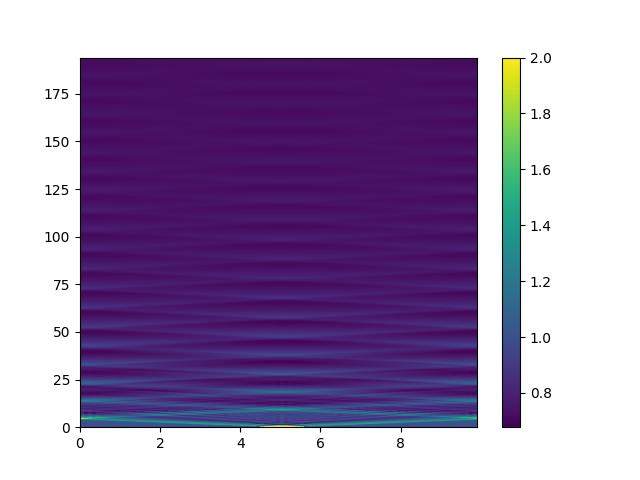
\includegraphics[width=\textwidth]{1/z_H_.jpg}  % Путь к первой картинке
		\caption{Изменение плотности}
	\end{minipage}%
	\hfill
	% Вторая картинка
	\begin{minipage}[b]{0.49\linewidth}
		\centering
		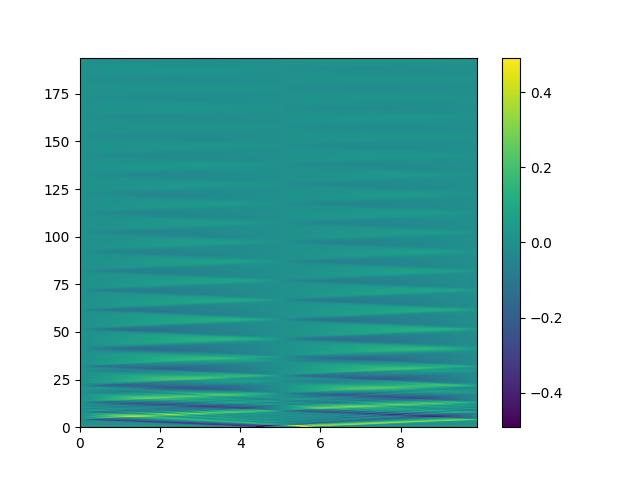
\includegraphics[width=\textwidth]{1/z_V_.jpg}  % Путь ко второй картинке
		\caption{Изменение скорости}
	\end{minipage}
	\caption{Графики для $\tau = 0.1, \ h = 0.1, \ C_{\rho} = 1, \ \mu = 0.1$}
	\label{ris:images}
\end{figure}

\begin{figure}[h]
	\begin{minipage}[h]{0.47\linewidth}
		\centering
		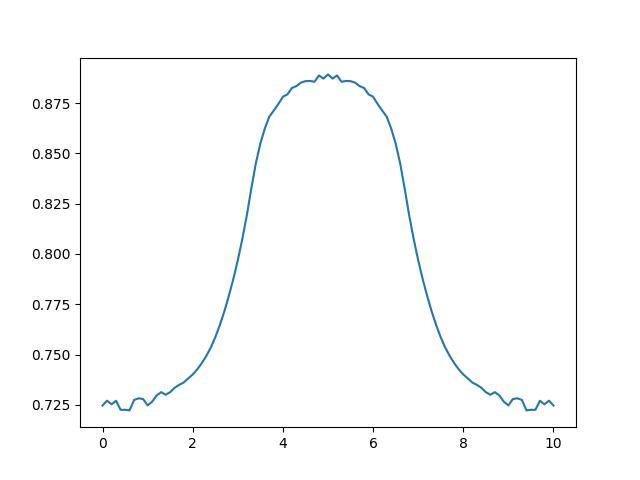
\includegraphics[width=1\linewidth]{1/z_H_nst4_.jpg} 
		\caption{Изменение плотности на слое $n_{st} / 4$}
	\end{minipage}
	\hfill
	\begin{minipage}[h]{0.47\linewidth}
		\centering
		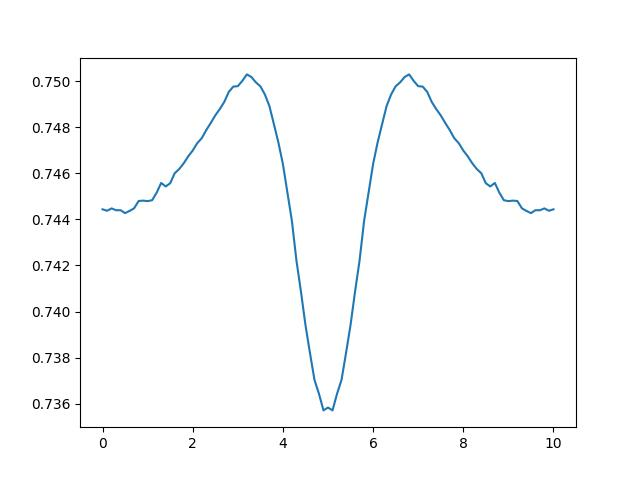
\includegraphics[width=1\linewidth]{1/z_H_nst2_.jpg} 
		\caption{Изменение плотности на слое $n_{st} / 2$}
	\end{minipage}
	\vfill
	\begin{minipage}[h]{0.47\linewidth}
		\centering
		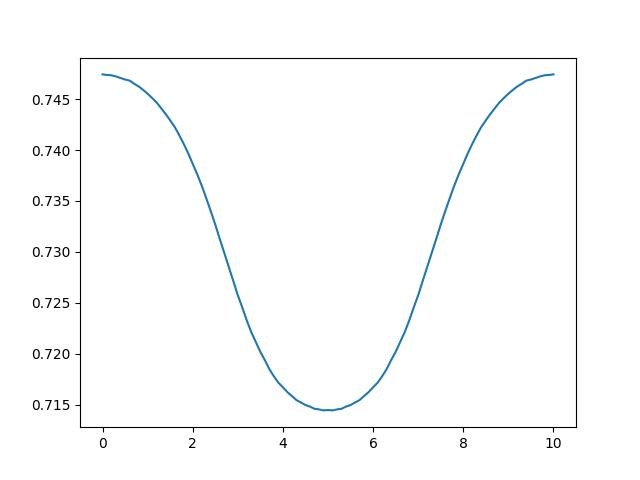
\includegraphics[width=1\linewidth]{1/z_H_3nst4_.jpg} 
		\caption{Изменение плотности на слое $3n_{st} / 4$}
	\end{minipage}
	\hfill
	\begin{minipage}[h]{0.47\linewidth}
		\centering
		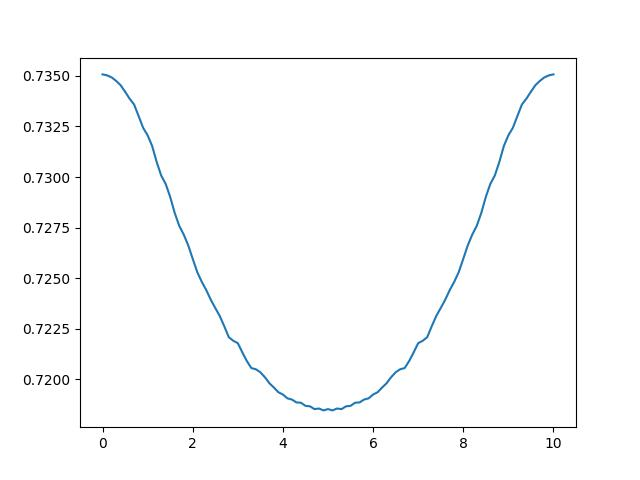
\includegraphics[width=1\linewidth]{1/z_H_nst_.jpg} 
		\caption{Изменение плотности на слое $n_{st}$}
	\end{minipage}
	\caption{Графики изменения плотности для $\tau = 0.1, \ h = 0.1, \ C_{\rho} = 1, \ \mu = 0.1$}
	\label{ris:experimentalcorrelationsignals}
\end{figure}

\begin{figure}[h]
	\begin{minipage}[h]{0.47\linewidth}
		\centering
		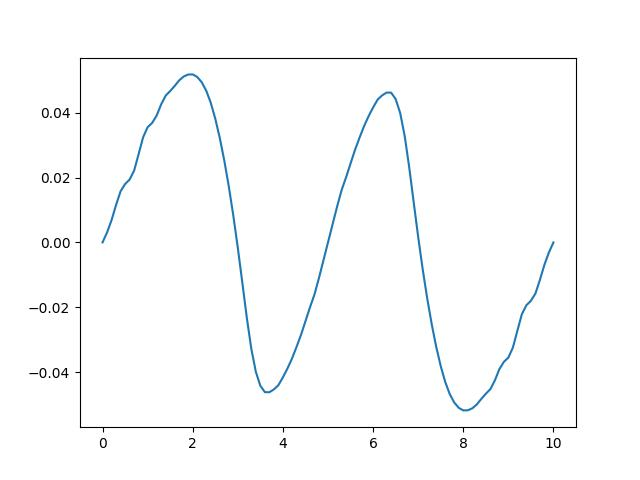
\includegraphics[width=1\linewidth]{1/z_V_nst4_.jpg} 
		\caption{Изменение скорости на слое $n_{st} / 4$}
	\end{minipage}
	\hfill
	\begin{minipage}[h]{0.47\linewidth}
		\centering
		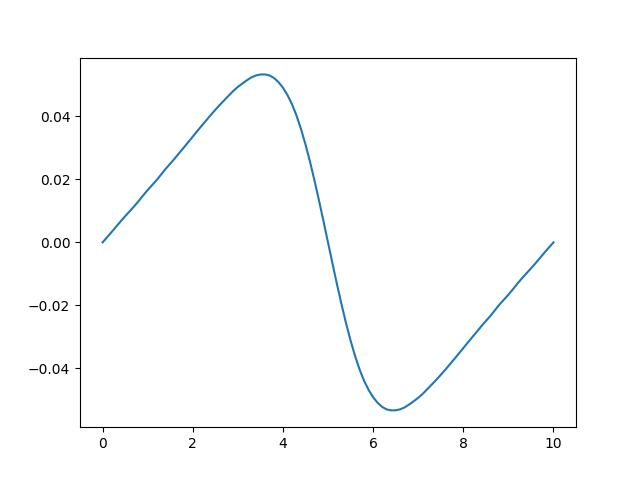
\includegraphics[width=1\linewidth]{1/z_V_nst2_.jpg} 
		\caption{Изменение скорости на слое $n_{st} / 2$}
	\end{minipage}
\end{figure}
\begin{figure}[h]
	\begin{minipage}[h]{0.47\linewidth}
		\centering
		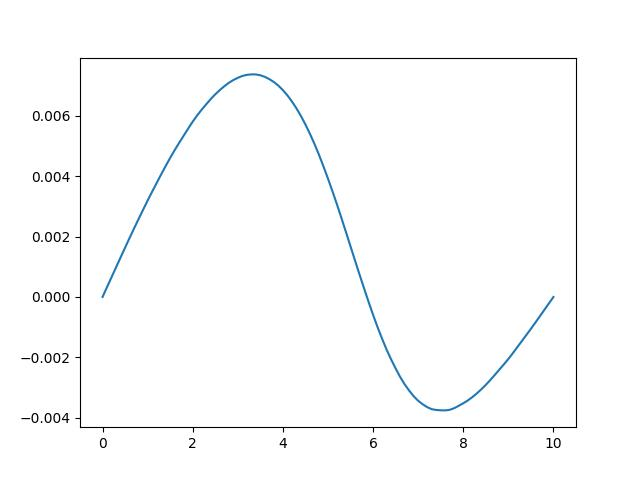
\includegraphics[width=1\linewidth]{2/z_V_3nst4_.jpg} 
		\caption{Изменение скорости на слое $3n_{st} / 4$}
	\end{minipage}
	\hfill
	\begin{minipage}[h]{0.47\linewidth}
		\centering
		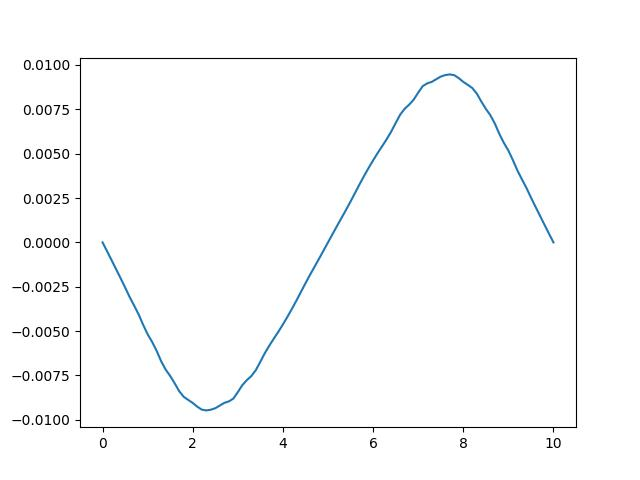
\includegraphics[width=1\linewidth]{1/z_V_nst_.jpg} 
		\caption{Изменение скорости на слое $n_{st}$}
	\end{minipage}
	\caption{Графики изменения скорости для $\tau = 0.1, \ h = 0.1, \ C_{\rho} = 1, \ \mu = 0.1$}
	\label{ris:experimentalcorrelationsignals}
\end{figure}

\begin{figure}[h]
	\centering
	% Первая картинка
	\begin{minipage}[b]{0.49\linewidth}
		\centering
		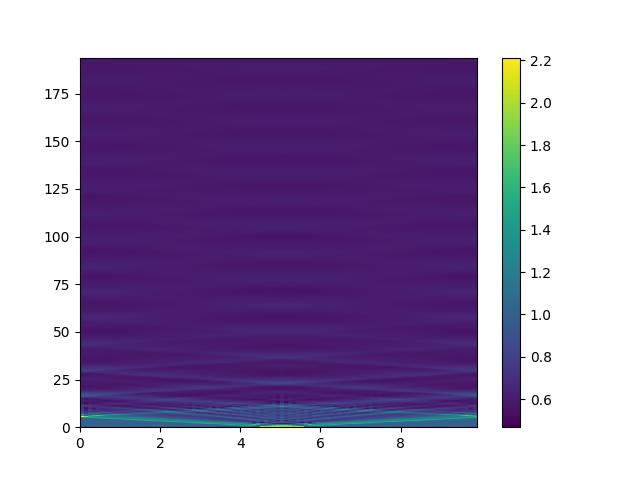
\includegraphics[width=\textwidth]{1/z_H_e.jpg}  % Путь к первой картинке
		\caption{Изменение плотности}
	\end{minipage}%
	\hfill
	% Вторая картинка
	\begin{minipage}[b]{0.49\linewidth}
		\centering
		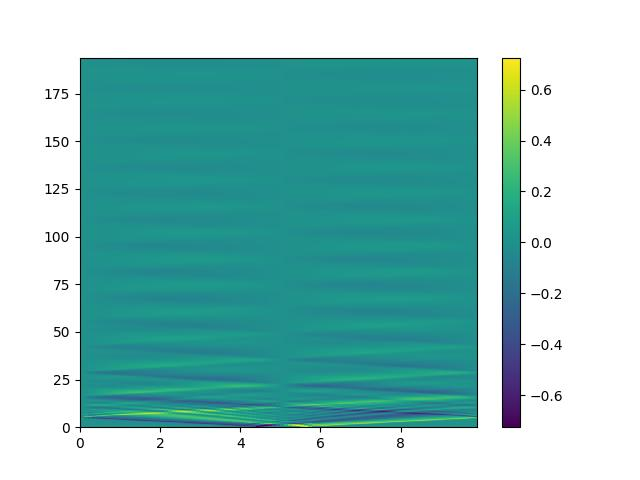
\includegraphics[width=\textwidth]{1/z_V_e.jpg}  % Путь ко второй картинке
		\caption{Изменение скорости}
	\end{minipage}
	\caption{Графики для $\tau = 0.1, \ h = 0.1, \ \gamma = 1.4, \ \mu = 0.1$}
	\label{ris:images}
\end{figure}

\begin{figure}[h]
	\begin{minipage}[h]{0.47\linewidth}
		\centering
		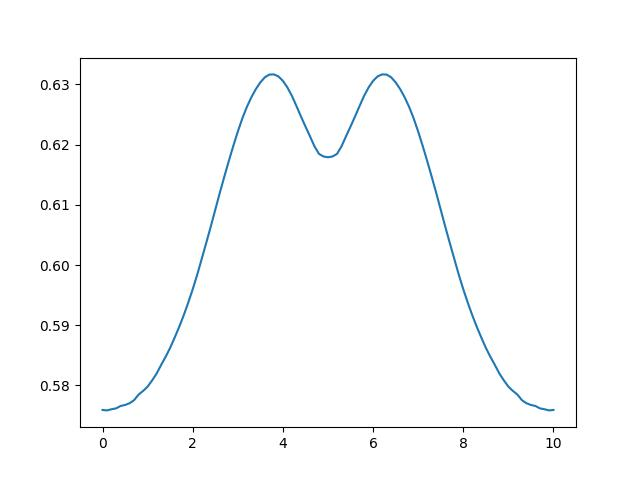
\includegraphics[width=1\linewidth]{1/z_H_nst4_e.jpg} 
		\caption{Изменение плотности на слое $n_{st} / 4$}
	\end{minipage}
	\hfill
	\begin{minipage}[h]{0.47\linewidth}
		\centering
		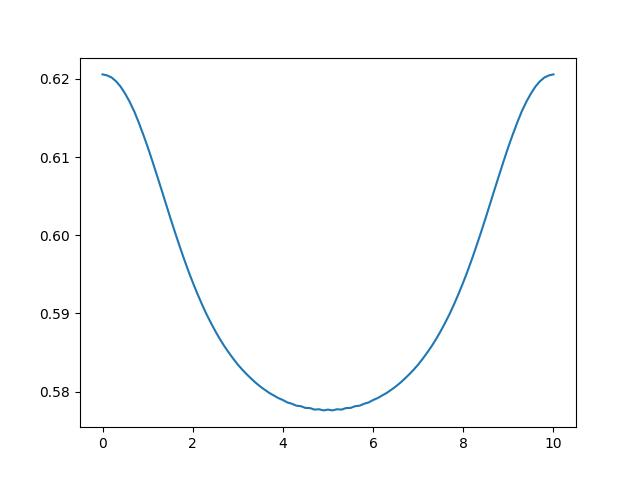
\includegraphics[width=1\linewidth]{1/z_H_nst2_e.jpg} 
		\caption{Изменение плотности на слое $n_{st} / 2$}
	\end{minipage}
\end{figure}
\begin{figure}[h]
	\begin{minipage}[h]{0.47\linewidth}
		\centering
		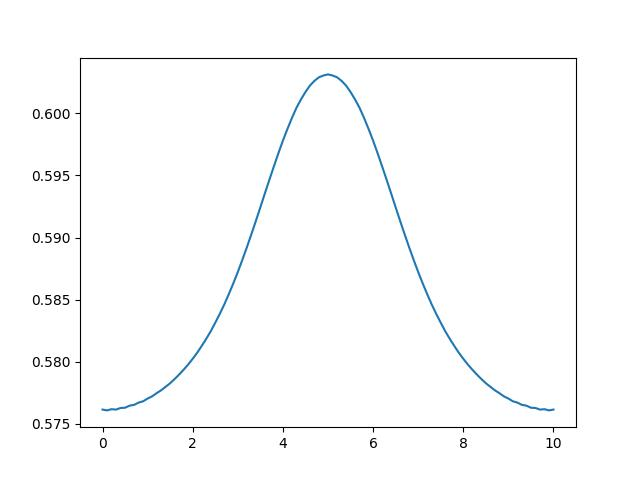
\includegraphics[width=1\linewidth]{1/z_H_3nst4_e.jpg} 
		\caption{Изменение плотности на слое $3n_{st} / 4$}
	\end{minipage}
	\hfill
	\begin{minipage}[h]{0.47\linewidth}
		\centering
		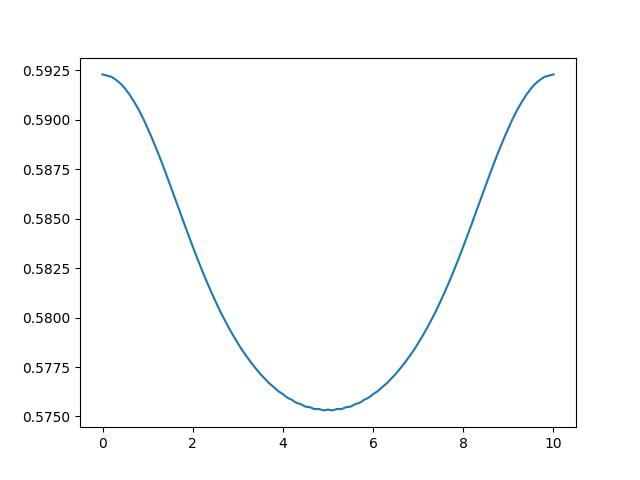
\includegraphics[width=1\linewidth]{1/z_H_nst_e.jpg} 
		\caption{Изменение плотности на слое $n_{st}$}
	\end{minipage}
	\caption{Графики изменения плотности для $\tau = 0.1, \ h = 0.1, \ \gamma = 1.4, \ \mu = 0.1$}
	\label{ris:experimentalcorrelationsignals}
\end{figure}

\begin{figure}[h]
	\begin{minipage}[h]{0.47\linewidth}
		\centering
		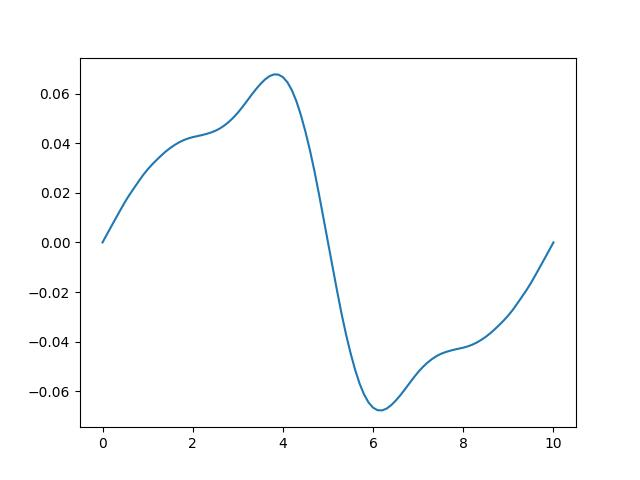
\includegraphics[width=1\linewidth]{1/z_V_nst4_e.jpg} 
		\caption{Изменение скорости на слое $n_{st} / 4$}
	\end{minipage}
	\hfill
	\begin{minipage}[h]{0.47\linewidth}
		\centering
		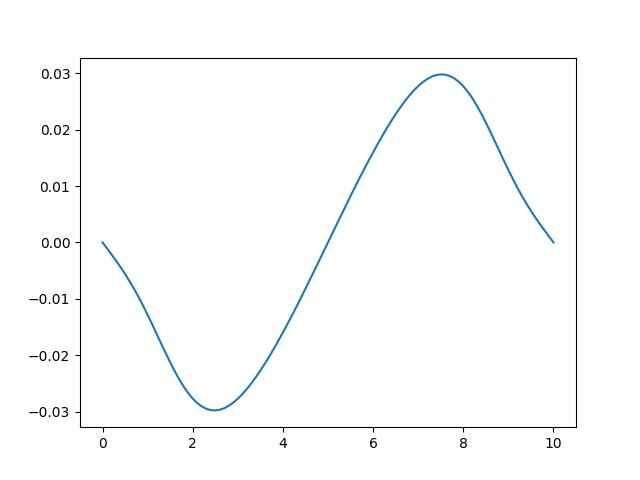
\includegraphics[width=1\linewidth]{1/z_V_nst2_e.jpg} 
		\caption{Изменение скорости на слое $n_{st} / 2$}
	\end{minipage}
	\vfill
	\begin{minipage}[h]{0.47\linewidth}
		\centering
		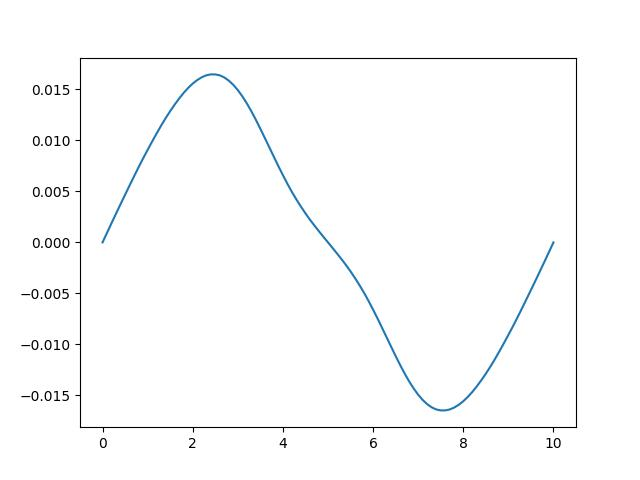
\includegraphics[width=1\linewidth]{1/z_V_3nst4_e.jpg} 
		\caption{Изменение скорости на слое $3n_{st} / 4$}
	\end{minipage}
	\hfill
	\begin{minipage}[h]{0.47\linewidth}
		\centering
		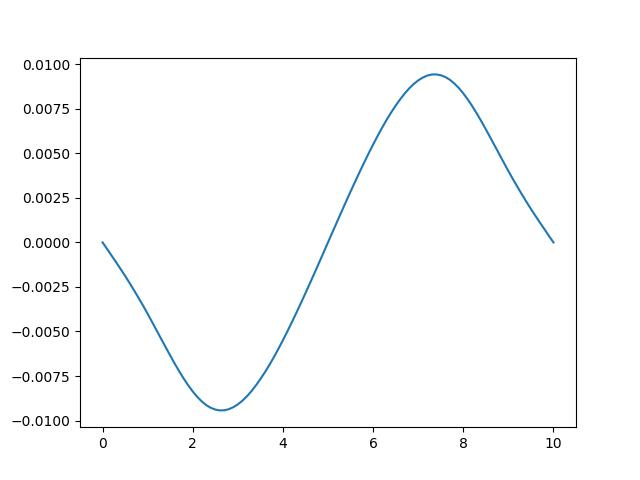
\includegraphics[width=1\linewidth]{1/z_V_nst_e.jpg} 
		\caption{Изменение скорости на слое $n_{st}$}
	\end{minipage}
	\caption{Графики изменения скорости для $\tau = 0.1, \ h = 0.1, \ \gamma = 1.4, \ \mu = 0.1$}
	\label{ris:experimentalcorrelationsignals}
\end{figure}

\clearpage
\newpage
Ниже приведены таблицы содержащие времена стабилизации $T_{st}$ решений второй системы и величин $|| (H^{n_{st}}, V^{n_{st}}) - (\tilde{H}, \tilde{V})||_{C_h}$ при различных входных параметрах (строки таблицы) на разных временных слоях (столбцы таблицы). Так же приведены таблицы, содержащие величины 
\begin{equation*}
	\displaystyle \Delta_m (n) = \frac{\sum\limits_{m \in \bar{\omega}_h} H^n_m - \sum\limits_{m \in \bar{\omega}_h} H^0_m}{\sum\limits_{m \in \bar{\omega}_h} H^0_m}
\end{equation*}
на разных временных слоях (столбцы таблицы) при различных входных параметрах (строки таблицы).
\subsubsection{Таблицы для второй системы}

1. $C_{\rho} = 1, \ \mu = 0.1$
\begin{center}
	\begin{tabular}{ |c|c|c|c|c|c| } 
		\hline
		$\tau$, h & $n_{st}/ 4$ & $n_{st}/ 2$ & $3n_{st}/ 4$ & $n_{st}$ & $T_{st}$ \\ 
		\hline
		1e-01, 1e-01 & 4.240e-03 & 7.926e-04 & 3.560e-04 & 4.980e-05 & 3252.0\\ 
		\hline
		1e-01, 1e-02 & 1.310e-02 & 7.075e-03 & 2.204e-03 & 9.584e-04 & 7230.2\\ 
		\hline
		1e-02, 1e-01 & 4.634e-03 & 3.106e-04 & 2.039e-05 & 9.994e-07 & 2295.54\\ 
		\hline
		1e-02, 1e-02 & 2.997e-02 & 9.378e-03 & 3.115e-03 & 9.982e-04 & 882.29\\ 
		\hline
	\end{tabular}
\end{center}

\begin{center}
	\begin{tabular}{ |c|c|c|c|c| } 
		\hline
		$\tau$, h & $\Delta_m (n_{st}/ 4)$ & $\Delta_m (n_{st}/ 2)$ & $\Delta_m (3n_{st}/ 4)$ & $\Delta_m (n_{st})$ \\ 
		\hline
		1e-01, 1e-01 & -3.188e-01 & -3.393e-01 & -3.432e-01 & -3.443e-01 \\ 
		\hline
		1e-01, 1e-02 & -1.515e-01 & -1.720e-01 & -2.209e-01 & -2.444e-01 \\ 
		\hline
		1e-02, 1e-01 & -9.427e-02 & -9.608e-02 & -9.620e-02 & -9.620e-02 \\ 
		\hline
		1e-02, 1e-02 & -8.733e-03 & -9.626e-03 & -9.917e-03 & -1.002e-02 \\ 
		\hline
	\end{tabular}
\end{center}

2. $C_{\rho} = 1, \ \mu = 0.01$
\begin{center}
	\begin{tabular}{ |c|c|c|c|c|c| } 
		\hline
		$\tau$, h & $n_{st}/ 4$ & $n_{st}/ 2$ & $3n_{st}/ 4$ & $n_{st}$ & $T_{st}$ \\ 
		\hline
		1e-02, 1e-01 & 2.420e-03 & 6.126e-05 & 2.775e-05 & 9.913e-07 & 4060.64\\ 
		\hline
		1e-02, 1e-02 & 5.016e-02 & 4.545e-02 & 2.405e-02 & 9.973e-03 & 691.75\\ 
		\hline
		1e-03, 1e-01 & 1.476e-02 & 3.562e-03 & 1.169e-03 & 1.999e-04 & 340.797\\ 
		\hline
		1e-03, 1e-02 & 1.348e-01 & 7.861e-02 & 8.904e-02 & 4.000e-02 & 147.892\\ 
		\hline
	\end{tabular}
\end{center}

\begin{center}
	\begin{tabular}{ |c|c|c|c|c| } 
		\hline
		$\tau$, h & $\Delta_m (n_{st}/ 4)$ & $\Delta_m (n_{st}/ 2)$ & $\Delta_m (3n_{st}/ 4)$ & $\Delta_m (n_{st})$ \\ 
		\hline
		1e-02, 1e-01 & -8.250e-01 & -8.255e-01 & -8.255e-01 & -8.256e-01 \\ 
		\hline
		1e-02, 1e-02 & -3.657e-01 & -3.758e-01 & -3.813e-01 & -3.840e-01 \\ 
		\hline
		1e-03, 1e-01 & -7.855e-01 & -7.927e-01 & -7.942e-01 & -7.947e-01 \\ 
		\hline
		1e-03, 1e-02 & -2.590e-02 & -5.641e-02 & -6.694e-02 & -7.169e-02 \\ 
		\hline
	\end{tabular}
\end{center}

3. $C_{\rho} = 1, \ \mu = 0.001$
\begin{center}
	\begin{tabular}{ |c|c|c|c|c|c| } 
		\hline
		$\tau$, h & $n_{st}/ 4$ & $n_{st}/ 2$ & $3n_{st}/ 4$ & $n_{st}$ & $T_{st}$ \\ 
		\hline
		1e-03, 1e-02 & 5.664e-02 & 3.272e-02 & 3.500e-02 & 9.999e-03 & 139.701\\ 
		\hline
		1e-04, 1e-02 & 6.939e-01 & 2.490e-01 & 1.204e-01 & 9.999e-02 & 17.5948\\ 
		\hline
		1e-04, 1e-03 & 2.482e-01 & 2.577e-01 & 1.324e-01 & 1.000e-01 & 57.4926\\ 
		\hline
		1e-04, 5e-03 & 4.866e-01 & 2.676e-01 & 7.889e-02 & 4.998e-02 & 21.5834\\ 
		\hline
	\end{tabular}
\end{center}

\begin{center}
	\begin{tabular}{ |c|c|c|c|c| } 
		\hline
		$\tau$, h & $\Delta_m (n_{st}/ 4)$ & $\Delta_m (n_{st}/ 2)$ & $\Delta_m (3n_{st}/ 4)$ & $\Delta_m (n_{st})$ \\ 
		\hline
		1e-03, 1e-02 & -8.179e-01 & -8.224e-01 & -8.238e-01 & -8.247e-01 \\ 
		\hline
		1e-04, 1e-02 & -4.119e-01 & -7.533e-01 & -7.759e-01 & -7.830e-01 \\ 
		\hline
		1e-04, 1e-03 & -2.018e-02 & -2.545e-02 & -3.370e-02 & -4.811e-02 \\ 
		\hline
		1e-04, 5e-03 & -4.506e-01 & -5.645e-01 & -5.845e-01 & -5.911e-01 \\ 
		\hline
	\end{tabular}
\end{center}

4. $C_{\rho} = 10, \ \mu = 0.1$
\begin{center}
	\begin{tabular}{ |c|c|c|c|c|c| } 
		\hline
		$\tau$, h & $n_{st}/ 4$ & $n_{st}/ 2$ & $3n_{st}/ 4$ & $n_{st}$ & $T_{st}$ \\ 
		\hline
		1e-02, 1e-01 & 1.717e-02 & 1.551e-02 & 2.266e-03 & 9.669e-05 & 294.1\\ 
		\hline
		1e-02, 1e-02 & 2.478e-01 & 1.978e-01 & 1.240e-01 & 4.969e-02 & 103.42\\ 
		\hline
		1e-03, 1e-01 & 1.225e-02 & 2.116e-02 & 8.215e-03 & 9.993e-04 & 426.676\\ 
		\hline
		1e-03, 1e-02 & 1.304e-01 & 5.164e-02 & 2.450e-02 & 9.996e-03 & 201.059\\ 
		\hline
	\end{tabular}
\end{center}

\begin{center}
	\begin{tabular}{ |c|c|c|c|c| } 
		\hline
		$\tau$, h & $\Delta_m (n_{st}/ 4)$ & $\Delta_m (n_{st}/ 2)$ & $\Delta_m (3n_{st}/ 4)$ & $\Delta_m (n_{st})$ \\ 
		\hline
		1e-02, 1e-01 & -5.727e-01 & -5.853e-01 & -5.886e-01 & -5.893e-01 \\ 
		\hline
		1e-02, 1e-02 & -1.299e-01 & -1.565e-01 & -1.701e-01 & -1.808e-01 \\ 
		\hline
		1e-03, 1e-01 & -3.722e-01 & -3.778e-01 & -3.805e-01 & -3.823e-01 \\ 
		\hline
		1e-03, 1e-02 & -4.720e-03 & -7.215e-03 & -8.229e-03 & -8.799e-03 \\ 
		\hline
	\end{tabular}
\end{center}

5. $C_{\rho} = 10, \ \mu = 0.01$
\begin{center}
	\begin{tabular}{ |c|c|c|c|c|c| } 
		\hline
		$\tau$, h & $n_{st}/ 4$ & $n_{st}/ 2$ & $3n_{st}/ 4$ & $n_{st}$ & $T_{st}$ \\ 
		\hline
		1e-02, 1e-01 & 4.589e-03 & 2.739e-04 & 1.559e-05 & 9.853e-11 & 3195.61\\ 
		\hline
		1e-03, 1e-01 & 8.293e-02 & 1.116e-02 & 4.091e-03 & 9.984e-04 & 239.415\\ 
		\hline
		1e-03, 1e-02 & 5.475e-02 & 2.402e-02 & 3.342e-02 & 9.995e-03 & 587.866\\ 
		\hline
		1e-03, 1e-03 & 2.966e-01 & 2.398e-01 & 1.548e-01 & 9.989e-02 & 24.231\\ 
		\hline
	\end{tabular}
\end{center}

\begin{center}
	\begin{tabular}{ |c|c|c|c|c| } 
		\hline
		$\tau$, h & $\Delta_m (n_{st}/ 4)$ & $\Delta_m (n_{st}/ 2)$ & $\Delta_m (3n_{st}/ 4)$ & $\Delta_m (n_{st})$ \\ 
		\hline
		1e-02, 1e-01 & -9.597e-01 & -9.598e-01 & -9.598e-01 & -9.598e-01 \\ 
		\hline
		1e-03, 1e-01 & -9.367e-01 & -9.378e-01 & -9.381e-01 & -9.381e-01 \\ 
		\hline
		1e-03, 1e-02 & -5.998e-01 & -6.013e-01 & -6.023e-01 & -6.032e-01 \\ 
		\hline
		1e-03, 1e-03 & -1.623e-01 & -1.799e-01 & -1.914e-01 & -2.007e-01 \\ 
		\hline
	\end{tabular}
\end{center}

6. $C_{\rho} = 10, \ \mu = 0.001$
\begin{center}
	\begin{tabular}{ |c|c|c|c|c|c| } 
		\hline
		$\tau$, h & $n_{st}/ 4$ & $n_{st}/ 2$ & $3n_{st}/ 4$ & $n_{st}$ & $T_{st}$ \\ 
		\hline
		1e-04, 1e-03 & 6.669e-01 & 2.933e-01 & 1.659e-01 & 9.989e-02 & 7.0227\\ 
		\hline
		1e-04, 1e-04 & 2.579e-01 & 1.760e-01 & 2.071e-01 & 9.990e-02 & 14.5659\\ 
		\hline
		1e-05, 1e-03 & 2.405e-01 & 1.236e-01 & 2.385e-01 & 9.995e-02 & 16.56307\\ 
		\hline
		1e-05, 1e-04 & 2.295e-01 & 1.683e-01 & 2.307e-01 & 9.936e-02 & 19.76507\\ 
		\hline
	\end{tabular}
\end{center}

\begin{center}
	\begin{tabular}{ |c|c|c|c|c| } 
		\hline
		$\tau$, h & $\Delta_m (n_{st}/ 4)$ & $\Delta_m (n_{st}/ 2)$ & $\Delta_m (3n_{st}/ 4)$ & $\Delta_m (n_{st})$ \\ 
		\hline
		1e-04, 1e-03 & -5.571e-01 & -5.926e-01 & -5.957e-01 & -5.972e-01 \\ 
		\hline
		1e-04, 1e-04 & -1.798e-01 & -2.108e-01 & -2.256e-01 & -2.343e-01 \\ 
		\hline
		1e-05, 1e-03 & -1.693e-01 & -2.403e-01 & -2.043e-01 & -1.939e-02 \\ 
		\hline
		1e-05, 1e-04 & -1.605e-01 & -1.466e-01 & -1.055e-01 & -1.909e-02 \\ 
		\hline
	\end{tabular}
\end{center}

7. $C_{\rho} = 100, \ \mu = 0.1$
\begin{center}
	\begin{tabular}{ |c|c|c|c|c|c| } 
		\hline
		$\tau$, h & $n_{st}/ 4$ & $n_{st}/ 2$ & $3n_{st}/ 4$ & $n_{st}$ & $T_{st}$ \\ 
		\hline
		1e-03, 1e-01 & 3.827e-02 & 7.681e-03 & 1.128e-03 & 9.777e-06 & 313.255\\ 
		\hline
		1e-04, 1e-01 & 6.820e-02 & 5.212e-02 & 2.006e-02 & 9.987e-04 & 115.2639\\ 
		\hline
		1e-03, 1e-02 & 1.705e-01 & 6.334e-02 & 4.986e-02 & 9.675e-03 & 137.214\\ 
		\hline
		1e-04, 1e-02 & 3.141e-01 & 2.386e-01 & 2.093e-01 & 9.994e-02 & 21.6863\\ 
		\hline
	\end{tabular}
\end{center}

\begin{center}
	\begin{tabular}{ |c|c|c|c|c| } 
		\hline
		$\tau$, h & $\Delta_m (n_{st}/ 4)$ & $\Delta_m (n_{st}/ 2)$ & $\Delta_m (3n_{st}/ 4)$ & $\Delta_m (n_{st})$ \\ 
		\hline
		1e-03, 1e-01 & -8.229e-01 & -8.242e-01 & -8.243e-01 & -8.244e-01 \\ 
		\hline
		1e-04, 1e-02 & -7.972e-01 & -7.980e-01 & -7.985e-01 & -7.988e-01 \\ 
		\hline
		1e-03, 1e-02 & -3.443e-01 & -3.494e-01 & -3.518e-01 & -3.572e-01 \\ 
		\hline
		1e-04, 1e-02 & -9.908e-04 & -1.712e-03 & -2.196e-03 & -2.684e-03 \\ 
		\hline
	\end{tabular}
\end{center}

8. $C_{\rho} = 100, \ \mu = 0.01$
\begin{center}
	\begin{tabular}{ |c|c|c|c|c|c| } 
		\hline
		$\tau$, h & $n_{st}/ 4$ & $n_{st}/ 2$ & $3n_{st}/ 4$ & $n_{st}$ & $T_{st}$ \\ 
		\hline
		1e-04, 1e-02 & 7.101e-01 & 4.201e-01 & 2.824e-01 & 1.000e-01 & 10.5744\\ 
		\hline
		1e-04, 1e-03 & 3.540e-01 & 2.302e-01 & 2.295e-01 & 9.967e-02 & 16.6095\\ 
		\hline
		1e-04, 1e-04 & 2.184e-01 & 1.949e-01 & 1.728e-01 & 9.954e-02 & 21.4930\\ 
		\hline
		1e-05, 1e-04 & 1.928e-01 & 1.749e-01 & 1.492e-01 & 9.902e-01 & 24.29384\\ 
		\hline
	\end{tabular}
\end{center}

\begin{center}
	\begin{tabular}{ |c|c|c|c|c| } 
		\hline
		$\tau$, h & $\Delta_m (n_{st}/ 4)$ & $\Delta_m (n_{st}/ 2)$ & $\Delta_m (3n_{st}/ 4)$ & $\Delta_m (n_{st})$ \\ 
		\hline
		1e-04, 1e-02 & -8.176e-01 & -8.225e-01 & -8.240e-01 & -8.247e-01 \\ 
		\hline
		1e-04, 1e-03 & -3.410e-01 & -3.484e-01 & -3.517e-01 & -3.535e-01 \\ 
		\hline
		1e-04, 1e-04 & -1.395e-01 & -2.403e-01 & -2.103e-01 & -1.249e-01 \\ 
		\hline
		1e-05, 1e-05 & -1.234e-01 & -1.339e-01 & -1.293e-01 & -1.111e-01 \\ 
		\hline
	\end{tabular}
\end{center}

9. $C_{\rho} = 100, \ \mu = 0.001$
\begin{center}
	\begin{tabular}{ |c|c|c|c|c|c| } 
		\hline
		$\tau$, h & $n_{st}/ 4$ & $n_{st}/ 2$ & $3n_{st}/ 4$ & $n_{st}$ & $T_{st}$ \\ 
		\hline
		1e-04, 1e-04 & 2.585e-01 & 1.255e-01 & 2.485e-01 & 9.245e-02 & 9.3575\\ 
		\hline
		1e-04, 1e-05 & 2.469e-01 & 1.757e-01 & 2.477e-01 & 9.945e-02 & 11.7436\\ 
		\hline
		1e-05, 1e-04 & 2.445e-01 & 1.256e-01 & 2.585e-01 & 9.995e-02 & 13.55678\\ 
		\hline
		1e-05, 1e-05 & 2.485e-01 & 2.3943e-01 & 1.049e-01 & 9.999e-02 & 20.54838\\ 
		\hline
	\end{tabular}
\end{center}

\begin{center}
	\begin{tabular}{ |c|c|c|c|c| } 
		\hline
		$\tau$, h & $\Delta_m (n_{st}/ 4)$ & $\Delta_m (n_{st}/ 2)$ & $\Delta_m (3n_{st}/ 4)$ & $\Delta_m (n_{st})$ \\ 
		\hline
		1e-04, 1e-04 & -1.394e-01 & -2.294e-01 & -2.294e-01 & -2.-295e-01 \\ 
		\hline
		1e-04, 1e-05 & -2.842e-01 & -1.283e-01 & -1.392e-01 & -1.384e-01 \\ 
		\hline
		1e-05, 1e-04 & -3.293-01 & -1.239e-01 & -1.395-01 & -8.294e-02 \\ 
		\hline
		1e-05, 1e-05 & -1.293e-01 & -1.120e-01 & -9.938e-02 & -9.834e-02 \\ 
		\hline
	\end{tabular}
\end{center}

10. $\gamma = 1.4, \ \mu = 0.1$
\begin{center}
	\begin{tabular}{ |c|c|c|c|c|c| } 
		\hline
		$\tau$, h & $n_{st}/ 4$ & $n_{st}/ 2$ & $3n_{st}/ 4$ & $n_{st}$ & $T_{st}$ \\ 
		\hline
		1e-01, 1e-01 & 4.558e-03 & 1.155e-03 & 7.850e-05 & 4.997e-05 & 2418.5\\ 
		\hline
		1e-01, 1e-02 & 1.670e-02 & 5.063e-03 & 2.587e-03 & 9.932e-04 & 1506.2\\ 
		\hline
		1e-02, 1e-01 & 2.175e-02 & 1.043e-02 & 2.862e-03 & 9.981e-04 & 816.63\\ 
		\hline
		1e-02, 1e-02 & 2.389e-02 & 7.778e-03 & 3.787e-03 & 9.966e-04 & 857.32\\ 
		\hline
	\end{tabular}
\end{center}

\begin{center}
	\begin{tabular}{ |c|c|c|c|c| } 
		\hline
		$\tau$, h & $\Delta_m (n_{st}/ 4)$ & $\Delta_m (n_{st}/ 2)$ & $\Delta_m (3n_{st}/ 4)$ & $\Delta_m (n_{st})$ \\ 
		\hline
		1e-01, 1e-01 & -4.140e-01 & -4.161e-01 & -4.171e-01 & -4.174e-01 \\ 
		\hline
		1e-01, 1e-02 & -3.476e-01 & -3.485e-01 & -3.488e-01 & -3.497e-01 \\ 
		\hline
		1e-02, 1e-01 & -9.636e-02 & -1.042e-01 & -1.067e-01 & -1.077e-01 \\ 
		\hline
		1e-02, 1e-02 & -9.308e-03 & -1.011e-02 & -1.038e-02 & -1.049e-02 \\ 
		\hline
	\end{tabular}
\end{center}

11. $\gamma = 1.4, \ \mu = 0.01$
\begin{center}
	\begin{tabular}{ |c|c|c|c|c|c| } 
		\hline
		$\tau$, h & $n_{st}/ 4$ & $n_{st}/ 2$ & $3n_{st}/ 4$ & $n_{st}$ & $T_{st}$ \\ 
		\hline
		1e-02, 1e-01 & 1.161e-02 & 1.348e-03 & 1.155e-03 & 9.970e-05 & 2531.09\\ 
		\hline
		1e-01, 1e-02 & 8.478e-03 & 3.473e-03 & 1.612e-03 & 9.908e-05 & 2396.1\\ 
		\hline
		1e-02, 1e-02 & 2.500e-02 & 2.242e-02 & 1.536e-02 & 9.997e-03 & 610.05\\ 
		\hline
		1e-03. 1e-01 & 6.304e-02 & 4.850e-02 & 2.548e-02 & 9.998e-03 & 358.151\\ 
		\hline
	\end{tabular}
\end{center}

\begin{center}
	\begin{tabular}{ |c|c|c|c|c| } 
		\hline
		$\tau$, h & $\Delta_m (n_{st}/ 4)$ & $\Delta_m (n_{st}/ 2)$ & $\Delta_m (3n_{st}/ 4)$ & $\Delta_m (n_{st})$ \\ 
		\hline
		1e-02, 1e-01 & -7.940e-01 & -7.962e-01 & -7.968e-01 & -7.970e-01 \\ 
		\hline
		1e-01, 1e-02 & -8.893e-01 & -8.895e-01 & -8.895e-01 & -8.895e-01 \\ 
		\hline
		1e-02, 1e-02 & -4.454e-01 & -4.491e-01 & -4.529e-01 & -4.550e-01 \\ 
		\hline
		1e-03, 1e-01 & -7.528e-01 & -7.597e-01 & -7.651e-01 & -7.679e-01 \\ 
		\hline
	\end{tabular}
\end{center}

12. $\gamma = 1.4, \ \mu = 0.001$
\begin{center}
	\begin{tabular}{ |c|c|c|c|c|c| } 
		\hline
		$\tau$, h & $n_{st}/ 4$ & $n_{st}/ 2$ & $3n_{st}/ 4$ & $n_{st}$ & $T_{st}$ \\ 
		\hline
		1e-03, 1e-02 & 5.632e-02 & 3.318e-02 & 2.946e-02 & 9.997e-03 & 150.266\\ 
		\hline
		1e-04, 1e-02 & 5.659e-01 & 3.775e-01 & 2.741e-01 & 9.999e-02 & 14.8061\\ 
		\hline
		1e-03, 1e-03 & 4.057e-01 & 2.019e-01 & 1.823e-01 & 9.993e-02 & 15.979\\ 
		\hline
		1e-02, 1e-03 & 8.980e-01 & 2.083e-01 & 2.025e-01 & 9.992e-02 & 46.83\\ 
		\hline
	\end{tabular}
\end{center}

\begin{center}
	\begin{tabular}{ |c|c|c|c|c| } 
		\hline
		$\tau$, h & $\Delta_m (n_{st}/ 4)$ & $\Delta_m (n_{st}/ 2)$ & $\Delta_m (3n_{st}/ 4)$ & $\Delta_m (n_{st})$ \\ 
		\hline
		1e-03, 1e-02 & -7.891e-01 & -7.921e-01 & -7.934e-01 & -7.941e-01 \\ 
		\hline
		1e-04, 1e-02 & -4.030e-01 & -7.212e-01 & -7.379e-01 & -7.591e-01 \\ 
		\hline
		1e-03, 1e-03 & -3.617e-01 & -4.172e-01 & -4.210e-01 & -4.239e-01 \\ 
		\hline
		1e-02, 1e-03 & -8.741e-01 & -8.791e-01 & -8.803e-01 & -8.809e-01 \\ 
		\hline
	\end{tabular}
\end{center}

\subsubsection{Графики для второй системы}

\begin{figure}[h]
	\centering
	% Первая картинка
	\begin{minipage}[b]{0.49\linewidth}
		\centering
		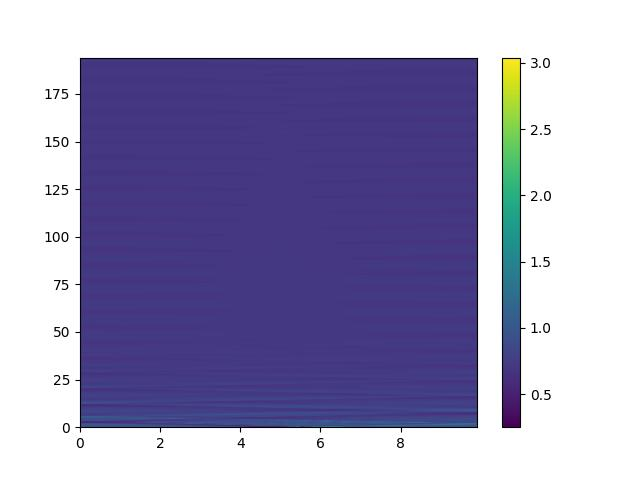
\includegraphics[width=\textwidth]{2/z_H_.jpg}  % Путь к первой картинке
		\caption{Изменение плотности}
	\end{minipage}%
	\hfill
	% Вторая картинка
	\begin{minipage}[b]{0.49\linewidth}
		\centering
		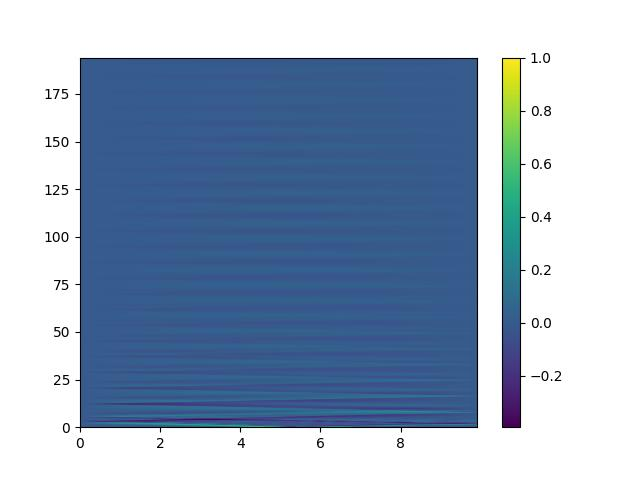
\includegraphics[width=\textwidth]{2/z_V_.jpg}  % Путь ко второй картинке
		\caption{Изменение скорости}
	\end{minipage}
	\caption{Графики для $\tau = 0.1, \ h = 0.1, \ C_{\rho} = 1, \ \mu = 0.1$}
	\label{ris:images}
\end{figure}

\begin{figure}[h]
	\begin{minipage}[h]{0.47\linewidth}
		\centering
		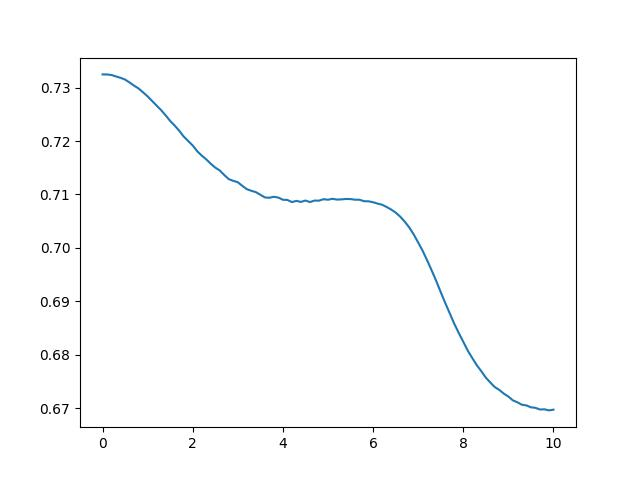
\includegraphics[width=1\linewidth]{2/z_H_nst4_.jpg} 
		\caption{Изменение плотности на слое $n_{st} / 4$}
	\end{minipage}
	\hfill
	\begin{minipage}[h]{0.47\linewidth}
		\centering
		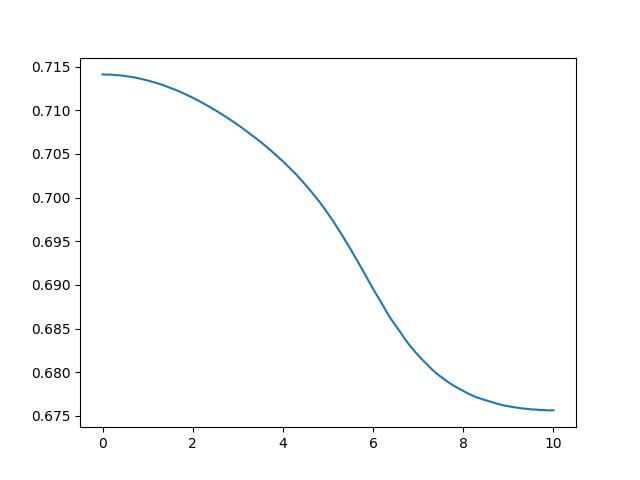
\includegraphics[width=1\linewidth]{2/z_H_nst2_.jpg} 
		\caption{Изменение плотности на слое $n_{st} / 2$}
	\end{minipage}
\end{figure}
\begin{figure}[h]
	\begin{minipage}[h]{0.47\linewidth}
		\centering
		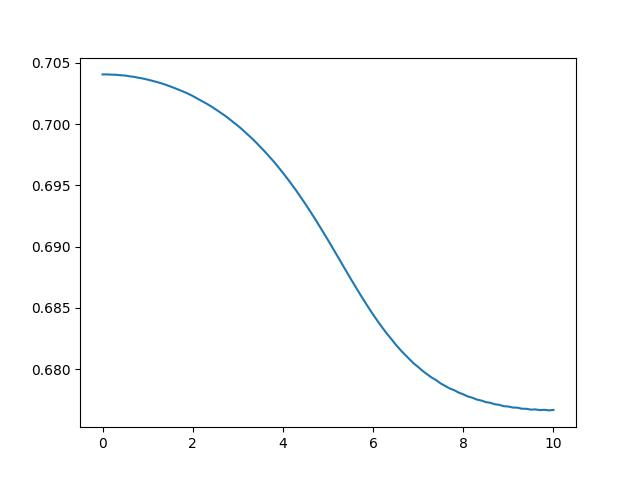
\includegraphics[width=1\linewidth]{2/z_H_3nst4_.jpg} 
		\caption{Изменение плотности на слое $3n_{st} / 4$}
	\end{minipage}
	\hfill
	\begin{minipage}[h]{0.47\linewidth}
		\centering
		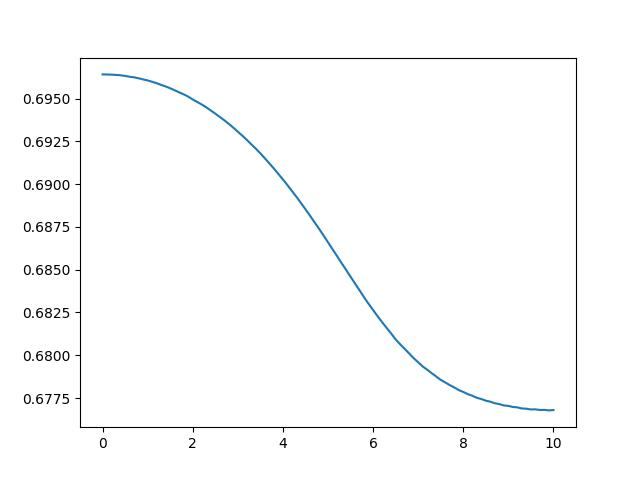
\includegraphics[width=1\linewidth]{2/z_H_nst_.jpg} 
		\caption{Изменение плотности на слое $n_{st}$}
	\end{minipage}
	\caption{Графики изменения плотности для $\tau = 0.1, \ h = 0.1, \ C_{\rho} = 1, \ \mu = 0.1$}
	\label{ris:experimentalcorrelationsignals}
\end{figure}

\begin{figure}[h]
	\begin{minipage}[h]{0.47\linewidth}
		\centering
		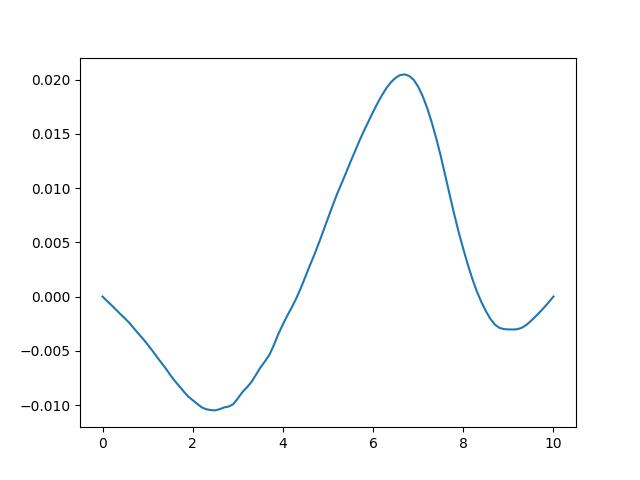
\includegraphics[width=1\linewidth]{2/z_V_nst4_.jpg} 
		\caption{Изменение скорости на слое $n_{st} / 4$}
	\end{minipage}
	\hfill
	\begin{minipage}[h]{0.47\linewidth}
		\centering
		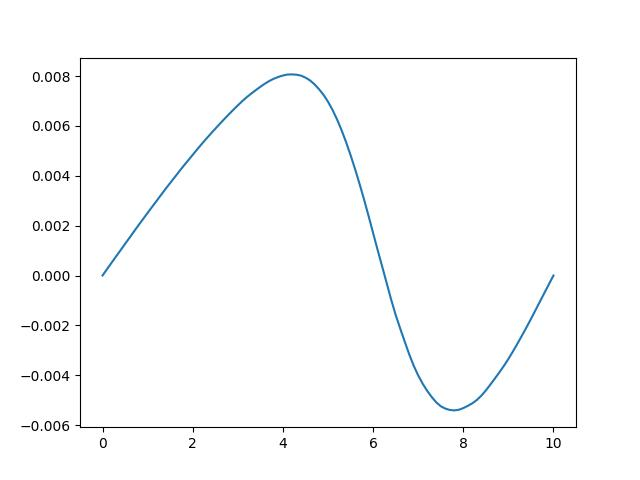
\includegraphics[width=1\linewidth]{2/z_V_nst2_.jpg} 
		\caption{Изменение скорости на слое $n_{st} / 2$}
	\end{minipage}
	\vfill
	\begin{minipage}[h]{0.47\linewidth}
		\centering
		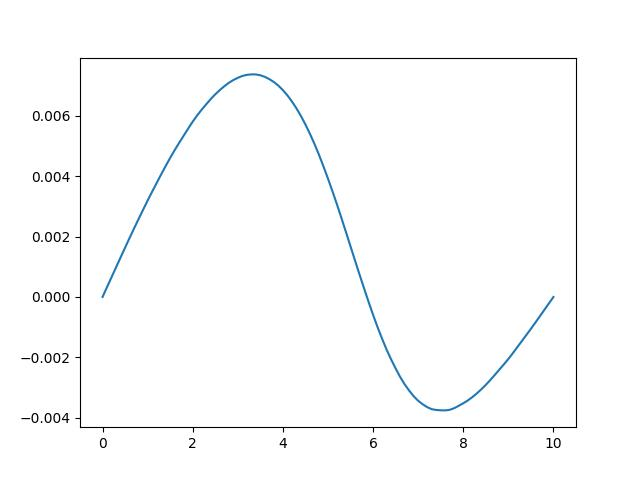
\includegraphics[width=1\linewidth]{2/z_V_3nst4_.jpg} 
		\caption{Изменение скорости на слое $3n_{st} / 4$}
	\end{minipage}
	\hfill
	\begin{minipage}[h]{0.47\linewidth}
		\centering
		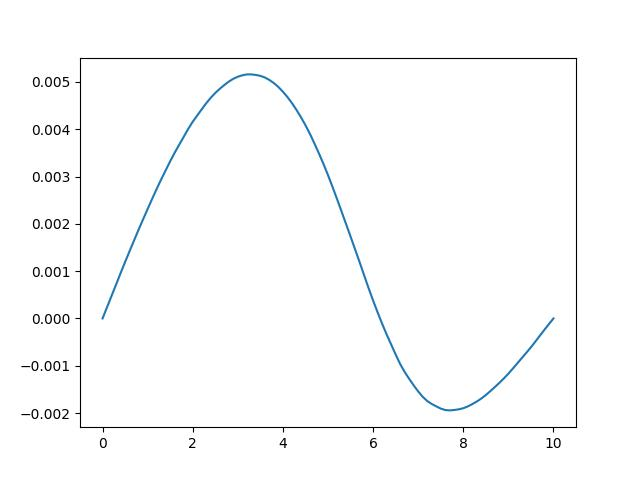
\includegraphics[width=1\linewidth]{2/z_V_nst_.jpg} 
		\caption{Изменение скорости на слое $n_{st}$}
	\end{minipage}
	\caption{Графики изменения скорости для $\tau = 0.1, \ h = 0.1, \ C_{\rho} = 1, \ \mu = 0.1$}
	\label{ris:experimentalcorrelationsignals}
\end{figure}

\begin{figure}[h]
	\centering
	% Первая картинка
	\begin{minipage}[b]{0.49\linewidth}
		\centering
		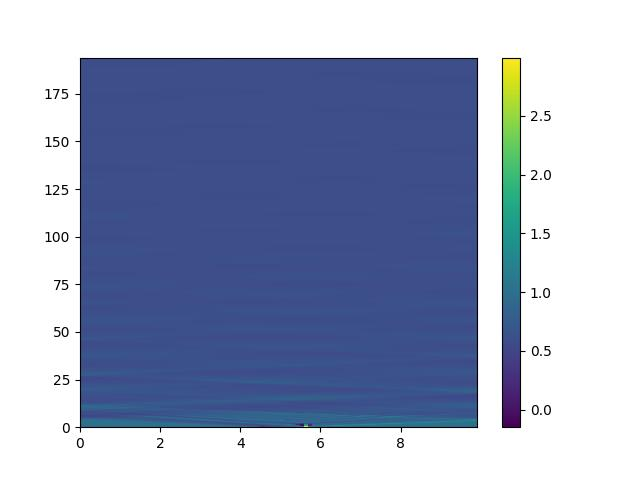
\includegraphics[width=\textwidth]{2/z_H_e.jpg}  % Путь к первой картинке
		\caption{Изменение плотности}
	\end{minipage}%
	\hfill
	% Вторая картинка
	\begin{minipage}[b]{0.49\linewidth}
		\centering
		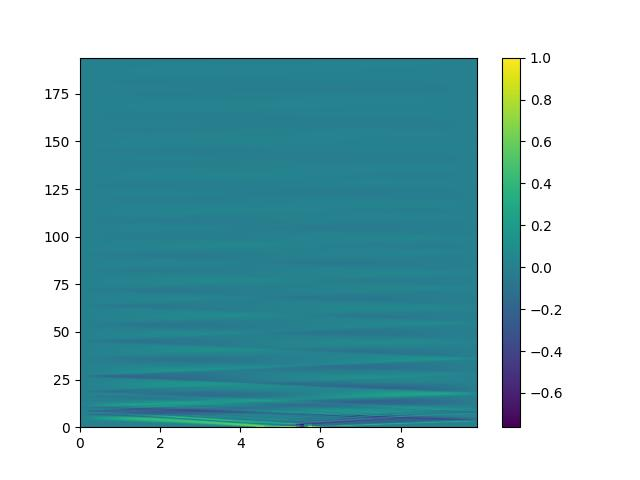
\includegraphics[width=\textwidth]{2/z_V_e.jpg}  % Путь ко второй картинке
		\caption{Изменение скорости}
	\end{minipage}
	\caption{Графики для $\tau = 0.1, \ h = 0.1, \ \gamma = 1.4, \ \mu = 0.1$}
	\label{ris:images}
\end{figure}

\begin{figure}[h]
	\begin{minipage}[h]{0.47\linewidth}
		\centering
		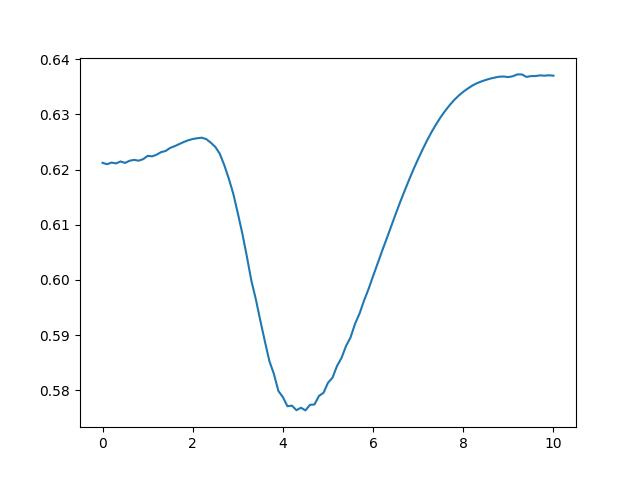
\includegraphics[width=1\linewidth]{2/z_H_nst4_e.jpg} 
		\caption{Изменение плотности на слое $n_{st} / 4$}
	\end{minipage}
	\hfill
	\begin{minipage}[h]{0.47\linewidth}
		\centering
		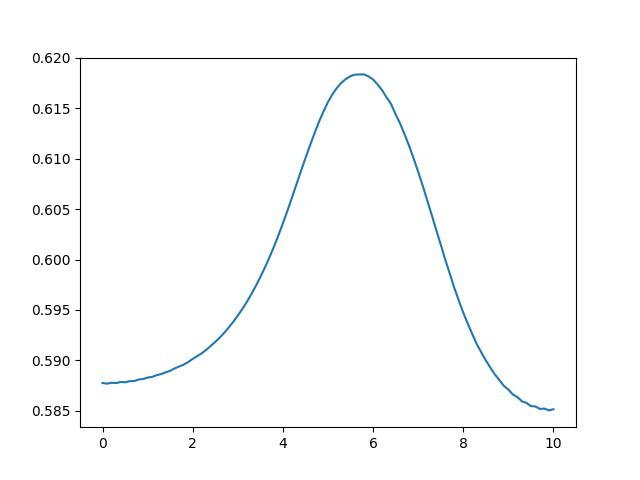
\includegraphics[width=1\linewidth]{2/z_H_nst2_e.jpg} 
		\caption{Изменение плотности на слое $n_{st} / 2$}
	\end{minipage}
	\vfill
	\begin{minipage}[h]{0.47\linewidth}
		\centering
		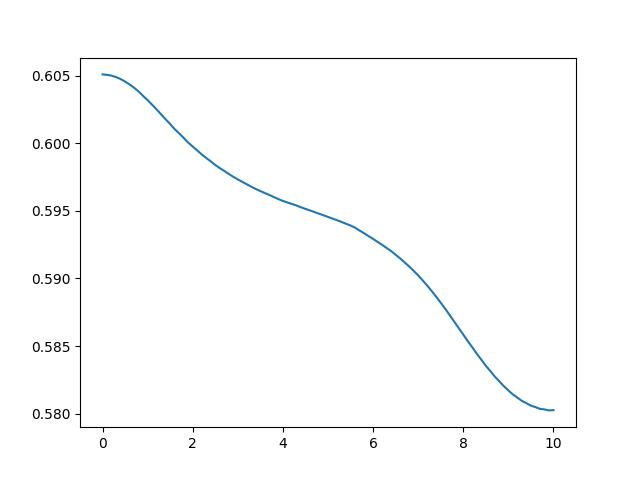
\includegraphics[width=1\linewidth]{2/z_H_3nst4_e.jpg} 
		\caption{Изменение плотности на слое $3n_{st} / 4$}
	\end{minipage}
	\hfill
	\begin{minipage}[h]{0.47\linewidth}
		\centering
		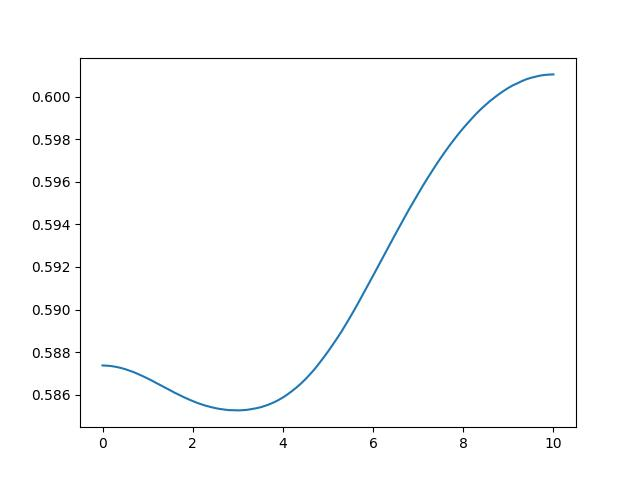
\includegraphics[width=1\linewidth]{2/z_H_nst_e.jpg} 
		\caption{Изменение плотности на слое $n_{st}$}
	\end{minipage}
	\caption{Графики изменения плотности для $\tau = 0.1, \ h = 0.1, \ \gamma = 1.4, \ \mu = 0.1$}
	\label{ris:experimentalcorrelationsignals}
\end{figure}

\begin{figure}[h]
	\begin{minipage}[h]{0.47\linewidth}
		\centering
		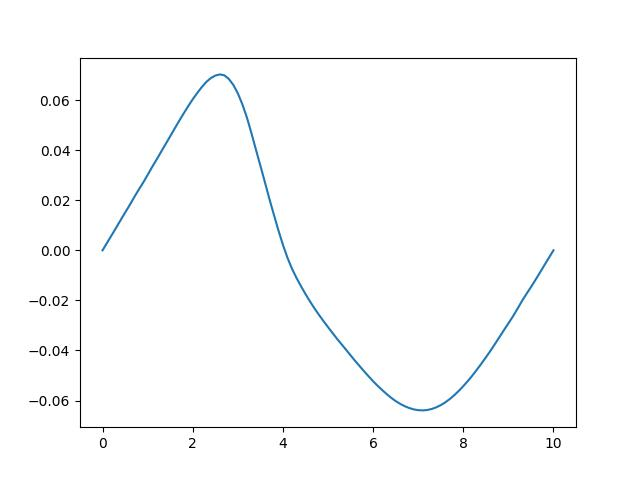
\includegraphics[width=1\linewidth]{2/z_V_nst4_e.jpg} 
		\caption{Изменение скорости на слое $n_{st} / 4$}
	\end{minipage}
	\hfill
	\begin{minipage}[h]{0.47\linewidth}
		\centering
		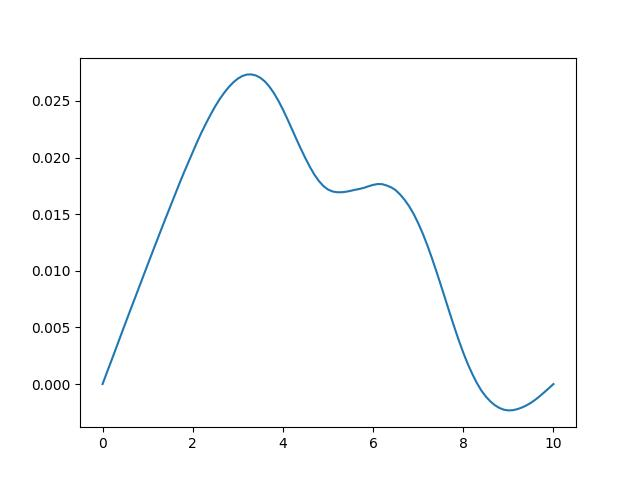
\includegraphics[width=1\linewidth]{2/z_V_nst2_e.jpg} 
		\caption{Изменение скорости на слое $n_{st} / 2$}
	\end{minipage}
	\vfill
	\begin{minipage}[h]{0.47\linewidth}
		\centering
		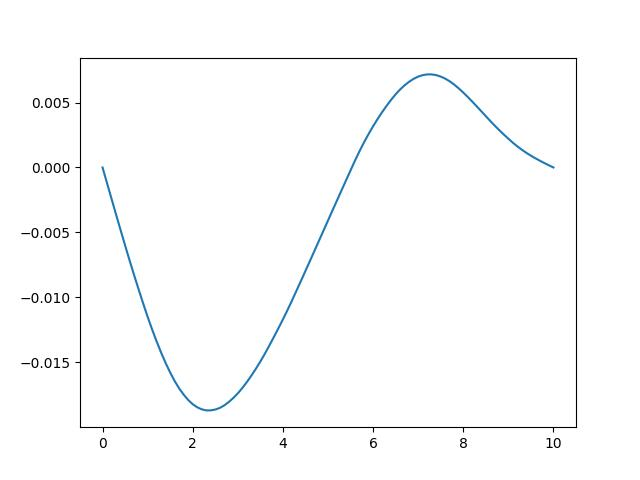
\includegraphics[width=1\linewidth]{2/z_V_3nst4_e.jpg} 
		\caption{Изменение скорости на слое $3n_{st} / 4$}
	\end{minipage}
	\hfill
	\begin{minipage}[h]{0.47\linewidth}
		\centering
		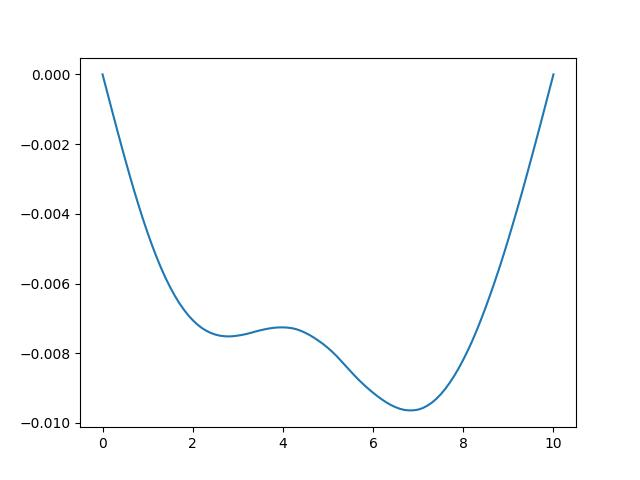
\includegraphics[width=1\linewidth]{2/z_V_nst_e.jpg} 
		\caption{Изменение скорости на слое $n_{st}$}
	\end{minipage}
	\caption{Графики изменения скорости для $\tau = 0.1, \ h = 0.1, \ \gamma = 1.4, \ \mu = 0.1$}
	\label{ris:experimentalcorrelationsignals}
\end{figure}

\section{Стабилизация осциллирующей функции}

Для системы (1) на области $Q = [0; T] \times [0, 1]$ зададим две задачи со следующими начальными и граничными условиями:
\begin{equation}
	\begin{cases}
		$$
		\rho_0 (x) = 2 + \sin (k \pi x), \ \ x \in [0; 1],
		\\
		u_0 (x) \equiv 0, \ \ x \in [0; 1], 
		\\
		u (t, 0) = u (t, 1) = 0, \ \ t \in [0; T], 
		\\
		f \equiv 0.
		$$
	\end{cases}
\end{equation}

\begin{equation}
	\begin{cases}
		$$
		\rho_0 (x) \equiv 1, \ \ x \in [0; 1], 
		\\
		u_0 (x) = \sin (k \pi x), \ \ x \in [0; 1],
		\\
		u (t, 0) = u (t, 1) = 0, \ \ t \in [0; T],
		\\
		f \equiv 0.
		$$
	\end{cases}
\end{equation}
Число $k$ задающее число колебаний начальной функции, является натуральным и для численного эксперимента выбирается из диапазона от 1 до $M / 10$, где $Mh = 1$.

\subsection{Результаты для первой системы}
Ниже приведены таблицы содержащие времена стабилизации решений первой системы при различных частотах колебаний (строки таблиц) и входных параметрах (столбцы таблиц). В случае несходимости за время $T = 5 \cdot 10^6 * \tau$ в таблицу заносится величина $|| (H^T, V^T) - (\tilde{H}, \tilde{V})||_{C_h}$
\subsubsection{Таблицы для линейного давления}
1. $C_{\rho} = 1, \ \mu = 0.1$
\begin{center}
	\begin{tabular}{ |c|c|c|c|c| } 
		\hline
		  & $\tau$ = 1e-02 & $\tau$ = 1e-02 & $\tau$ = 5e-03 & $\tau$ = 1e-04 \\ 
		k & $h$ = 2e-03 & $h$ = 1e-03 & $h$ = 1e-03 & $h$ = 2e-03 \\ 
		  & $\varepsilon$ = 1e-05 & $\varepsilon$ = 1e-06 & $\varepsilon$ = 1e-01 & $\varepsilon$ = 1e-01 \\ 
		\hline
		1 & 17.46 & 21.91 & 0.725 & 0.7140 \\
		\hline
		2 & 51.81 & 63.83 & 5.610 & 5.4136 \\
		\hline
		3 & 14.91 & 18.06 & 1.350 & 1.2899 \\
		\hline
		4 & 47.82 & 59.85 & 2.410 & 2.3889 \\
		\hline
		5 & 12.97 & 16.42 & 0.685 & 0.6762 \\
		\hline
		6 & 45.82 & 57.84 & 1.335 & 0.6421 \\
		\hline
		7 & 12.40 & 21.58 & 0.650 & 0.3781 \\
		\hline
		8 & 44.75 & 56.77 & 0.580 & 0.4229 \\
		\hline
		9 & 17.95 & 21.13 & 0.250 & 0.2230 \\
		\hline
		10 & 43.72 & 55.73 & 0.400 & 0.3632 \\
		\hline
		$10 + M/10$ & 54.34 & 58.42 & 1.490 & 1.5297 \\
		\hline
		$10 + 2M/10$ & 49.77 & 62.20 & 2.425 & 3.3233 \\
		\hline
		$10 + 3M/10$ & 51.79 & 64.03 & 3.415 & 3.5866 \\
		\hline
		$10 + 4M/10$ & 55.76 & 60.17 & 3.575 & 3.5075 \\
		\hline
		$10 + 5M/10$ & 52.55 & 57.88 & 4.510 & 2.5624 \\
		\hline
		$10 + 6M/10$ & 47.90 & 58.53 & 4.460 & 8.4792 \\
		\hline
		$10 + 7M/10$ & 47.97 & 54.22 & 18.715 & 3.173e-01 \\
		\hline
		$10 + 8M/10$ & 52.06 & 59.81 & 1.869e-01 & 5.561e-01 \\
		\hline
		$10 + 9M/10$ & 47.63 & 63.65 & 14.190 & 2.732e-01 \\
		\hline
	\end{tabular}
\end{center}

2. $C_{\rho} = 1, \ \mu = 0.01$
\begin{center}
	\begin{tabular}{ |c|c|c|c|c| } 
		\hline
		 & $\tau$ = 1e-03 & $\tau$ = 1e-04 & $\tau$ = 1e-04 & $\tau$ = 5e-04 \\ 
		k & $h$ = 2e-03 & $h$ = 2e-03 & $h$ = 1e-03 & $h$ = 1e-03 \\ 
		& $\varepsilon$ = 1e-02 & $\varepsilon$ = 1e-01 & $\varepsilon$ = 1e-01 & $\varepsilon$ = 1e-02 \\ 
		\hline
		1 & 31.787 & 4.7548 & 4.7484 & 29.7495 \\
		\hline
		2 & 76.504 & 14.5186 & 15.4931 & 74.6755 \\
		\hline
		3 & 27.927 & 6.3052 & 6.3462 & 27.2775 \\
		\hline
		4 & 61.493 & 10.0576 & 11.0111 & 60.4455 \\
		\hline
		5 & 25.805 & 3.2883 & 3.2921 & 25.1590 \\
		\hline
		6 & 59.459 & 7.4621 & 8.4653 & 58.4255 \\
		\hline
		7 & 22.640 & 2.1304 & 2.1283 & 21.7585 \\
		\hline
		8 & 57.453 & 3.4150 & 3.5930 & 56.4230 \\
		\hline
		9 & 19.766 & 1.5768 & 1.5750 & 19.2575 \\
		\hline
		10 & 55.450 & 2.4192 & 2.4292 & 54.4215 \\
		\hline
		$10 + M/10$ & 6.764 & 0.1030 & 0.0378 & 2.4505 \\
		\hline
		$10 + 2M/10$ & 12.689 & 0.8354 & 1.1249 & 14.7125 \\
		\hline
		$10 + 3M/10$ & 18.472 & 1.1616 & 1.2547 & 13.4200 \\
		\hline
		$10 + 4M/10$ & 23.687 & 1.1149 & 1.7991 & 9.2485 \\
		\hline
		$10 + 5M/10$ & 46.560 & 3.5314 & 1.8544 & 13.3480 \\
		\hline
		$10 + 6M/10$ & 14.563 & 2.0991 & 2.0868 & 14.7820 \\
		\hline
		$10 + 7M/10$ & 23.699 & 3.0446 & 3.0482 & 25.6155 \\
		\hline
		$10 + 8M/10$ & 37.751 & 3.1495 & 2.7959 & 20.8750 \\
		\hline
		$10 + 9M/10$ & 20.770 & 2.6386 & 1.9094 & 43.6845 \\
		\hline
	\end{tabular}
\end{center}

3. $C_{\rho} = 1, \ \mu = 0.001$
\begin{center}
	\begin{tabular}{ |c|c|c|c|c| } 
		\hline
		& $\tau$ = 1e-03 & $\tau$ = 1e-04 & $\tau$ = 5e-04 & $\tau$ = 1e-04 \\ 
		k & $h$ = 2e-03 & $h$ = 2e-03 & $h$ = 1e-03 & $h$ = 5e-04 \\ 
		& $\varepsilon$ = 1e-02 & $\varepsilon$ = 1e-01 & $\varepsilon$ = 1e-01 & $\varepsilon$ = 1e-01 \\ 
		\hline
		1 & 38.183 & 1.9538 & 1.1945 & 7.3535 \\
		\hline
		2 & 39.666 & 2.2820 & 1.6280 & 15.2001 \\
		\hline
		3 & 35.353 & 2.6535 & 1.4360 & 8.4028 \\
		\hline
		4 & 25.888 & 1.6113 & 1.2770 & 9.0857 \\
		\hline
		5 & 16.788 & 1.2674 & 1.0205 & 5.0989 \\
		\hline
		6 & 17.150 & 3.4950 & 0.9875 & 7.9724 \\
		\hline
		7 & 19.172 & 1.5890 & 1.3265 & 3.7077 \\
		\hline
		8 & 39.880 & 2.8148 & 1.0195 & 7.9224 \\
		\hline
		9 & 6.775 & 1.2786 & 0.9945 & 3.0449 \\
		\hline
		10 & 14.495 & 1.5790 & 0.7990 & 4.3973 \\
		\hline
		$10 + M/10$ & 76.558 & 0.9824 & 0.1445 & 0.0782 \\
		\hline
		$10 + 2M/10$ & 18.089 & 0.1360 & 0.0795 & 0.0223 \\
		\hline
		$10 + 3M/10$ & 20.586 & 0.2029 & 0.5020 & 0.0666 \\
		\hline
		$10 + 4M/10$ & 43.675 & 9.291e-01 & 1.0325 & 0.0676 \\
		\hline
		$10 + 5M/10$ & 65.479 & 5.0282 & 2.5970 & 0.8232 \\
		\hline
		$10 + 6M/10$ & 1.184e+00 & 9.037e-01 & 1.003e+00 & 1.5006 \\
		\hline
		$10 + 7M/10$ & 1.760e+00 & 1.580e+00 & 1.436e+00 & 1.0886 \\
		\hline
		$10 + 8M/10$ & 1.660e+00 & 1.521e+00 & 1.623e+00 & 1.384e+00 \\
		\hline
		$10 + 9M/10$ & 9.965e-01 & 3.3156 & 1.800e+00 & 3.7862 \\
		\hline
	\end{tabular}
\end{center}

4. $C_{\rho} = 10, \ \mu = 0.1$
\begin{center}
	\begin{tabular}{ |c|c|c|c|c| } 
		\hline
		& $\tau$ = 1e-03 & $\tau$ = 1e-03 & $\tau$ = 1e-04 & $\tau$ = 1e-04 \\ 
		k & $h$ = 2e-03 & $h$ = 1e-03 & $h$ = 2e-03 & $h$ = 1e-03 \\ 
		& $\varepsilon$ = 1e-06 & $\varepsilon$ = 1e-06 & $\varepsilon$ = 1e-02 & $\varepsilon$ = 1e-02 \\ 
		\hline
		1 & 22.284 & 22.441 & 4.5580 & 4.5573 \\
		\hline
		2 & 60.693 & 61.950 & 13.8702 & 14.1800 \\
		\hline
		3 & 17.877 & 18.191 & 4.2585 & 4.3197 \\
		\hline
		4 & 58.790 & 60.049 & 11.9696 & 12.2802 \\
		\hline
		5 & 16.272 & 16.587 & 3.4458 & 3.4465 \\
		\hline
		6 & 57.839 & 58.785 & 11.0184 & 11.3292 \\
		\hline
		7 & 15.479 & 15.793 & 2.9712 & 2.9718 \\
		\hline
		8 & 56.890 & 57.837 & 10.0700 & 10.3811 \\
		\hline
		9 & 15.005 & 15.319 & 2.6570 & 2.6571 \\
		\hline
		10 & 55.941 & 57.201 & 9.4344 & 9.5480 \\
		\hline
		$10 + M/10$ & 46.759 & 44.539 & 3.1028 & 1.9542 \\
		\hline
		$10 + 2M/10$ & 42.612 & 41.672 & 4.0860 & 3.1247 \\
		\hline
		$10 + 3M/10$ & 42.733 & 43.011 & 5.7101 & 4.5191 \\
		\hline
		$10 + 4M/10$ & 40.820 & 39.219 & 6.3286 & 5.6862 \\
		\hline
		$10 + 5M/10$ & 37.964 & 38.283 & 6.6381 & 5.0424 \\
		\hline
		$10 + 6M/10$ & 30.599 & 32.219 & 4.0214 & 5.0030 \\
		\hline
		$10 + 7M/10$ & 29.095 & 31.914 & 5.9776 & 5.9672 \\
		\hline
		$10 + 8M/10$ & 30.953 & 33.800 & 5.3472 & 4.4730 \\
		\hline
		$10 + 9M/10$ & 37.381 & 40.450 & 5.8048 & 3.2954 \\
		\hline
	\end{tabular}
\end{center}

5. $C_{\rho} = 10, \ \mu = 0.01$
\begin{center}
	\begin{tabular}{ |c|c|c|c|c| } 
		\hline
		& $\tau$ = 1e-04 & $\tau$ = 1e-04 & $\tau$ = 5e-04 & $\tau$ = 1e-05 \\ 
		k & $h$ = 1e-03 & $h$ = 5e-04 & $h$ = 1e-03 & $h$ = 1e-03 \\ 
		& $\varepsilon$ = 1e-01 & $\varepsilon$ = 1e-01 & $\varepsilon$ = 1e-01 & $\varepsilon$ = 1e-01 \\ 
		\hline
		1 & 3.5024 & 3.4949 & 2.1420 & 3.34366 \\
		\hline
		2 & 7.6242 & 7.9234 & 7.9745 & 7.61603 \\
		\hline
		3 & 3.3554 & 3.5056 & 2.2655 & 3.35084 \\
		\hline
		4 & 5.6694 & 5.9750 & 4.8435 & 5.66509 \\
		\hline
		5 & 2.9937 & 3.1490 & 1.2990 & 2.99446 \\
		\hline
		6 & 5.3387 & 5.6454 & 3.5820 & 5.34101 \\
		\hline
		7 & 2.5132 & 2.8227 & 1.5920 & 2.51371 \\
		\hline
		8 & 5.0182 & 5.3234 & 3.7945 & 5.01758 \\
		\hline
		9 & 2.1945 & 2.3498 & 1.2670 & 2.19473 \\
		\hline
		10 & 4.6972 & 5.0063 & 2.4900 & 4.69679 \\
		\hline
		$10 + M/10$ & 0.1185 & 0.0307 & 0.1605 & 0.09929 \\
		\hline
		$10 + 2M/10$ & 0.0672 & 0.0667 & 0.1575 & 0.06722 \\
		\hline
		$10 + 3M/10$ & 0.3259 & 0.1494 & 0.4750 & 0.33204 \\
		\hline
		$10 + 4M/10$ & 0.3302 & 0.1523 & 0.6315 & 0.65298 \\
		\hline
		$10 + 5M/10$ & 2.5879 & 0.6813 & 0.1845 & 2.26993 \\
		\hline
		$10 + 6M/10$ & 1.7660 & 1.0955 & 1.9340 & 3.06858 \\
		\hline
		$10 + 7M/10$ & 3.2027 & 0.6533 & 4.2390 & 2.88987 \\
		\hline
		$10 + 8M/10$ & 2.1505 & 2.2650 & 1.053e+00 & 1.85450 \\
		\hline
		$10 + 9M/10$ & 0.7546 & 1.9480 & 3.0715 & 2.70235 \\
		\hline
	\end{tabular}
\end{center}

6. $C_{\rho} = 10, \ \mu = 0.001$
\begin{center}
	\begin{tabular}{ |c|c|c|c|c| } 
		\hline
		& $\tau$ = 1e-04 & $\tau$ = 1e-05 & $\tau$ = 5e-05 & $\tau$ = 1e-05 \\ 
		k & $h$ = 1e-03 & $h$ = 1e-03 & $h$ = 5e-04 & $h$ = 5e-04 \\ 
		& $\varepsilon$ = 1e-01 & $\varepsilon$ = 1e-01 & $\varepsilon$ = 1e-01 & $\varepsilon$ = 1e-01 \\ 
		\hline
		1 & 0.7789 & 1.33488 & 0.42920 & 0.68980 \\
		\hline
		2 & 1.5725 & 1.07607 & 1.08125 & 1.94834 \\
		\hline
		3 & 1.5833 & 1.53315 & 0.78770 & 1.44948 \\
		\hline
		4 & 3.0267 & 1.34601 & 1.00785 & 1.28141 \\
		\hline
		5 & 0.7868 & 2.68394 & 0.79120 & 0.81510 \\
		\hline
		6 & 1.1550 & 1.46809 & 0.80880 & 1.97537 \\
		\hline
		7 & 1.4537 & 1.41667 & 0.63320 & 1.58144 \\
		\hline
		8 & 0.8064 & 1.44629 & 0.49545 & 1.48196 \\
		\hline
		9 & 1.8436 & 1.22115 & 0.82190 & 0.48201 \\
		\hline
		10 & 0.9795 & 0.87727 & 0.66530 & 0.67729 \\
		\hline
		$10 + M/10$ & 1.4440 & 0.35822 & 0.32905 & 0.20877 \\
		\hline
		$10 + 2M/10$ & 4.154e+00 & 0.81572 & 0.10535 & 0.04272 \\
		\hline
		$10 + 3M/10$ & 9.745e+00 & 2.63880 & 1.57550 & 0.30586 \\
		\hline
		$10 + 4M/10$ & 4.784e+00 & 4.713e+00 & 1.858e+00 & 1.739e+00 \\
		\hline
		$10 + 5M/10$ & 1.182e+01 & 3.97638 & 0.62945 & 2.51722 \\
		\hline
		$10 + 6M/10$ & 5.275e+00 & 4.266e+00 & 2.259e+00 & 1.001e+00 \\
		\hline
		$10 + 7M/10$ & 5.724e+00 & 7.684e+00 & 3.775e+00 & 3.476e+00 \\
		\hline
		$10 + 8M/10$ & 6.993e+00 & 8.243e+00 & 4.090e+00 & 3.929e+00 \\
		\hline
		$10 + 9M/10$ & 6.008e+00 & 5.29932 & 2.432e+00 & 1.02671 \\
		\hline
	\end{tabular}
\end{center}

7. $C_{\rho} = 100, \ \mu = 0.1$
\begin{center}
	\begin{tabular}{ |c|c|c|c|c| } 
		\hline
		& $\tau$ = 5e-04 & $\tau$ = 1e-04 & $\tau$ = 1e-04 & $\tau$ = 5e-04 \\ 
		k & $h$ = 2e-03 & $h$ = 2e-03 & $h$ = 1e-03 & $h$ = 1e-03 \\ 
		& $\varepsilon$ = 1e-02 & $\varepsilon$ = 1e-02 & $\varepsilon$ = 1e-02 & $\varepsilon$ = 1e-02 \\ 
		\hline
		1 & 12.9210 & 4.7556 & 4.9021 & 26.0945 \\
		\hline
		2 & 15.9400 & 10.4100 & 11.0044 & 17.3300 \\
		\hline
		3 & 7.5850 & 3.8091 & 4.0062 & 6.2280 \\
		\hline
		4 & 17.0595 & 8.9094 & 9.4040 & 21.4675 \\
		\hline
		5 & 4.5870 & 3.4966 & 3.6945 & 9.3710 \\
		\hline
		6 & 18.4315 & 8.7053 & 9.1044 & 27.0585 \\
		\hline
		7 & 5.5605 & 3.0933 & 3.3416 & 8.6015 \\
		\hline
		8 & 21.1945 & 8.5054 & 9.0006 & 39.3745 \\
		\hline
		9 & 5.7000 & 2.8427 & 3.0415 & 7.3045 \\
		\hline
		10 & 22.0025 & 8.4041 & 8.8027 & 37.5700 \\
		\hline
		$10 + M/10$ & 4.0950 & 3.2109 & 1.4093 & 4.9945 \\
		\hline
		$10 + 2M/10$ & 4.4875 & 3.0269 & 3.0063 & 5.0855 \\
		\hline
		$10 + 3M/10$ & 4.1855 & 3.4860 & 4.0999 & 5.7870 \\
		\hline
		$10 + 4M/10$ & 3.7855 & 3.9987 & 1.9056 & 4.9895 \\
		\hline
		$10 + 5M/10$ & 5.3045 & 5.7232 & 3.1305 & 3.5050 \\
		\hline
		$10 + 6M/10$ & 4.3255 & 2.0092 & 1.6524 & 2.0155 \\
		\hline
		$10 + 7M/10$ & 2.0870 & 2.6877 & 3.0057 & 4.7020 \\
		\hline
		$10 + 8M/10$ & 5.5900 & 4.1991 & 2.8074 & 3.5595 \\
		\hline
		$10 + 9M/10$ & 5.6840 & 2.8031 & 2.8683 & 6.9005 \\
		\hline
	\end{tabular}
\end{center}

8. $C_{\rho} = 100, \ \mu = 0.01$
\begin{center}
	\begin{tabular}{ |c|c|c|c|c| } 
		\hline
		& $\tau$ = 1e-04 & $\tau$ = 1e-05 & $\tau$ = 1e-05 & $\tau$ = 1e-04 \\ 
		k & $h$ = 1e-03 & $h$ = 1e-03 & $h$ = 1e-04 & $h$ = 1e-04 \\ 
		& $\varepsilon$ = 1e-01 & $\varepsilon$ = 1e-01 & $\varepsilon$ = 1e-01 & $\varepsilon$ = 1e-01 \\ 
		\hline
		1 & 4.3691 & 1.50594 & 3.70559 & 3.1792 \\
		\hline
		2 & 3.5320 & 7.04025 & 8.10615 & 7.3920 \\
		\hline
		3 & 1.5339 & 3.27959 & 3.65889 & 4.1784 \\
		\hline
		4 & 3.0896 & 4.91236 & 5.89255 & 6.5964 \\
		\hline
		5 & 1.9667 & 1.60471 & 3.64647 & 1.5542 \\
		\hline
		6 & 1.4803 & 5.64622 & 5.12293 & 4.480e+00 \\
		\hline
		7 & 1.0724 & 2.04933 & 3.64067 & 2.8040 \\
		\hline
		8 & 1.5738 & 4.59533 & 5.11234 & 8.1303 \\
		\hline
		9 & 0.8698 & 2.04306 & 3.58738 & 2.7108 \\
		\hline
		10 & 1.6436 & 4.33656 & 5.00517 & 7.2900 \\
		\hline
		$10 + M/10$ & 0.3551 & 0.19976 & 0.01443 & 0.2003 \\
		\hline
		$10 + 2M/10$ & 0.1483 & 0.09894 & 0.01508 & 0.0495 \\
		\hline
		$10 + 3M/10$ & 6.305e-01 & 0.30570 & 0.09197 & 0.4446 \\
		\hline
		$10 + 4M/10$ & 5.2064 & 0.69470 & 0.04865 & 0.2953 \\
		\hline
		$10 + 5M/10$ & 2.0495 & 5.40655 & 0.05614 & 0.2129 \\
		\hline
		$10 + 6M/10$ & 6.643e+00 & 2.435e+00 & 0.70300 & 0.0851 \\
		\hline
		$10 + 7M/10$ & 8.264e+00 & 5.312e+00 & 0.40698 & 1.114e+00 \\
		\hline
		$10 + 8M/10$ & 7.539e+00 & 4.26357 & 0.49585 & 0.2980 \\
		\hline
		$10 + 9M/10$ & 5.970e+00 & 3.83869 & 1.11423 & 1.1499 \\
		\hline
	\end{tabular}
\end{center}

9. $C_{\rho} = 100, \ \mu = 0.001$
\begin{center}
	\begin{tabular}{ |c|c|c|c|c| } 
		\hline
		& $\tau$ = 5e-06 & $\tau$ = 1e-05 & $\tau$ = 1e-06 & $\tau$ = 2e-06 \\ 
		k & $h$ = 1e-04 & $h$ = 1e-04 & $h$ = 1e-04 & $h$ = 1e-04 \\ 
		& $\varepsilon$ = 1e-01 & $\varepsilon$ = 1e-01 & $\varepsilon$ = 1e-01 & $\varepsilon$ = 1e-01 \\ 
		\hline
		1 & 0.353630 & 1.22607 & 0.394006 & 0.536772 \\
		\hline
		2 & 0.798470 & 0.91072 & 9.040487 & 8.938674 \\
		\hline
		3 & 0.649470 & 1.18107 & 4.430953 & 4.381892 \\
		\hline
		4 & 0.565575 & 1.29306 & 6.607547 & 6.604986 \\
		\hline
		5 & 0.503845 & 1.34779 & 4.458449 & 4.357776 \\
		\hline
		6 & 0.841715 & 0.75041 & 5.897728 & 5.893678 \\
		\hline
		7 & 0.813610 & 1.20375 & 3.245369 & 3.448014 \\
		\hline
		8 & 0.601440 & 0.91988 & 5.591423 & 5.587520 \\
		\hline
		9 & 0.871820 & 1.26518 & 3.343144 & 2.545554 \\
		\hline
		10 & 0.500850 & 1.28245 & 5.388953 & 2.880734 \\
		\hline
		$10 + M/10$ & 0.404260 & 0.75578 & 0.098193 & 0.097948 \\
		\hline
		$10 + 2M/10$ & 0.025645 & 0.04019 & 0.041557 & 0.026454 \\
		\hline
		$10 + 3M/10$ & 0.049610 & 5.99490 & 0.101324 & 0.101314 \\
		\hline
		$10 + 4M/10$ & 1.976975 & 8.90853 & 0.790752 & 1.139104 \\
		\hline
		$10 + 5M/10$ & 0.506660 & 7.30295 & 1.015760 & 1.104866 \\
		\hline
		$10 + 6M/10$ & 4.634e+00 & 5.577e+00 & 2.567e+00 & 3.118e+00 \\
		\hline
		$10 + 7M/10$ & 6.446e+00 & 7.539e+00 & 4.716e+00 & 5.846e+00 \\
		\hline
		$10 + 8M/10$ & 6.128e+00 & 6.634e+00 & 9.429e+00 & 6.721e+00 \\
		\hline
		$10 + 9M/10$ & 8.360e+00 & 7.421e+00 & 3.533303 & 2.501e+00 \\
		\hline
	\end{tabular}
\end{center}

\subsubsection{Таблицы для нелинейного давления}
1. $\gamma = 1.4, \ \mu = 0.1$
\begin{center}
	\begin{tabular}{ |c|c|c|c|c| } 
		\hline
		& $\tau$ = 1e-02 & $\tau$ = 1e-03 & $\tau$ = 1e-03 & $\tau$ = 1e-04 \\ 
		k & $h$ = 2e-03 & $h$ = 2e-03 & $h$ = 1e-03 & $h$ = 1e-03 \\ 
		& $\varepsilon$ = 1e-04 & $\varepsilon$ = 1e-04 & $\varepsilon$ = 1e-04 & $\varepsilon$ = 1e-04 \\ 
		\hline
		1 & 21.30 & 10.712 & 10.710 & 10.2605 \\
		\hline
		2 & 48.61 & 33.737 & 33.717 & 32.9525 \\
		\hline
		3 & 15.23 & 9.585 & 9.578 & 9.2131 \\
		\hline
		4 & 45.64 & 30.800 & 31.224 & 30.0216 \\
		\hline
		5 & 13.10 & 8.290 & 8.291 & 7.9331 \\
		\hline
		6 & 43.44 & 29.319 & 29.747 & 28.5443 \\
		\hline
		7 & 12.05 & 7.608 & 7.828 & 7.5610 \\
		\hline
		8 & 41.96 & 28.310 & 28.531 & 27.5367 \\
		\hline
		9 & 11.34 & 7.254 & 7.475 & 7.2080 \\
		\hline
		10 & 40.50 & 27.118 & 27.541 & 26.7940 \\
		\hline
		$10 + M/10$ & 28.85 & 39.770 & 19.674 & 19.7352 \\
		\hline
		$10 + 2M/10$ & 25.37 & 34.509 & 32.677 & 31.2668 \\
		\hline
		$10 + 3M/10$ & 26.27 & 34.776 & 24.718 & 29.2658 \\
		\hline
		$10 + 4M/10$ & 25.32 & 32.207 & 31.814 & 31.6360 \\
		\hline
		$10 + 5M/10$ & 25.30 & 30.947 & 22.682 & 31.8778 \\
		\hline
		$10 + 6M/10$ & 20.86 & 19.722 & 20.695 & 21.1532 \\
		\hline
		$10 + 7M/10$ & 24.29 & 1.227e-04 & 4.460e-02 & 9.443e-02 \\
		\hline
		$10 + 8M/10$ & 23.84 & 1.859e-01 & 1.624e-01 & 3.227e-01 \\
		\hline
		$10 + 9M/10$ & 41.12 & 7.376e-02 & 1.143e-01 & 3.228e-01 \\
		\hline
	\end{tabular}
\end{center}

2. $\gamma = 1.4, \ \mu = 0.01$
\begin{center}
	\begin{tabular}{ |c|c|c|c|c| } 
		\hline
		& $\tau$ = 1e-03 & $\tau$ = 1e-04 & $\tau$ = 1e-04 & $\tau$ = 1e-04 \\ 
		k & $h$ = 2e-03 & $h$ = 2e-03 & $h$ = 1e-03 & $h$ = 2e-03 \\ 
		& $\varepsilon$ = 1e-01 & $\varepsilon$ = 1e-01 & $\varepsilon$ = 1e-01 & $\varepsilon$ = 1e-01 \\ 
		\hline
		1 & 5.490 & 5.0856 & 5.0647 & 5.0856 \\
		\hline
		2 & 10.574 & 11.2186 & 11.1405 & 11.2186 \\
		\hline
		3 & 5.237 & 5.6975 & 5.6536 & 5.6975 \\
		\hline
		4 & 6.027 & 6.7086 & 6.6692 & 6.7086 \\
		\hline
		5 & 3.171 & 3.1448 & 3.1213 & 3.1448 \\
		\hline
		6 & 5.967 & 5.9403 & 6.6174 & 5.9403 \\
		\hline
		7 & 2.354 & 2.2586 & 2.3149 & 2.2586 \\
		\hline
		8 & 3.272 & 4.4544 & 4.4363 & 4.4544 \\
		\hline
		9 & 1.743 & 1.5689 & 1.6340 & 1.5689 \\
		\hline
		10 & 2.487 & 2.4508 & 3.2041 & 2.4508 \\
		\hline
		$10 + M/10$ & 0.136 & 0.0987 & 0.0342 & 0.0987 \\
		\hline
		$10 + 2M/10$ & 0.074 & 0.5760 & 0.6543 & 0.5760 \\
		\hline
		$10 + 3M/10$ & 0.657 & 0.9330 & 0.8408 & 0.9330 \\
		\hline
		$10 + 4M/10$ & 0.540 & 0.8809 & 0.8586 & 0.8809 \\
		\hline
		$10 + 5M/10$ & 1.022 & 3.4760 & 0.8697 & 3.4760 \\
		\hline
		$10 + 6M/10$ & 1.914 & 1.8543 & 1.7591 & 1.8543 \\
		\hline
		$10 + 7M/10$ & 8.186e-01 & 5.0956 & 2.8092 & 5.0956 \\
		\hline
		$10 + 8M/10$ & 1.339e+00 & 1.8573 & 2.5503 & 1.8573 \\
		\hline
		$10 + 9M/10$ & 2.590 & 2.7127 & 1.5284 & 2.7127 \\
		\hline
	\end{tabular}
\end{center}

3. $\gamma = 1.4, \ \mu = 0.001$
\begin{center}
	\begin{tabular}{ |c|c|c|c|c| } 
		\hline
		& $\tau$ = 1e-04 & $\tau$ = 1e-04 & $\tau$ = 5e-05 & $\tau$ = 1e-05 \\ 
		k & $h$ = 1e-03 & $h$ = 5e-04 & $h$ = 5e-04 & $h$ = 1e-04 \\ 
		& $\varepsilon$ = 1e-01 & $\varepsilon$ = 1e-01 & $\varepsilon$ = 1e-01 & $\varepsilon$ = 1e-01 \\ 
		\hline
		1 & 1.4275 & 0.3903 & 2.02875 & 6.30888 \\
		\hline
		2 & 2.4928 & 8.6602 & 9.30695 & 11.13878 \\
		\hline
		3 & 1.5311 & 4.6901 & 4.99550 & 6.21977 \\
		\hline
		4 & 2.1208 & 6.9362 & 6.87665 & 8.15964 \\
		\hline
		5 & 0.8066 & 2.9123 & 3.46710 & 6.18472 \\
		\hline
		6 & 1.2727 & 3.6867 & 5.32305 & 6.61519 \\
		\hline
		7 & 0.8021 & 2.3438 & 2.68595 & 4.38358 \\
		\hline
		8 & 0.9970 & 2.8589 & 4.57270 & 6.58666 \\
		\hline
		9 & 0.6008 & 1.9484 & 2.38390 & 3.29715 \\
		\hline
		10 & 0.9050 & 2.5504 & 3.60485 & 5.83328 \\
		\hline
		$10 + M/10$ & 0.1259 & 0.0640 & 0.06315 & 0.00396 \\
		\hline
		$10 + 2M/10$ & 0.0570 & 0.0233 & 0.02255 & 0.05756 \\
		\hline
		$10 + 3M/10$ & 0.2225 & 0.0324 & 0.03375 & 0.16295 \\
		\hline
		$10 + 4M/10$ & 0.9870 & 0.2016 & 0.13515 & 0.04605 \\
		\hline
		$10 + 5M/10$ & 1.9722 & 2.2755 & 2.71535 & 0.27939 \\
		\hline
		$10 + 6M/10$ & 1.034e+00 & 1.077e+00 & 2.182e+00 & 0.54332 \\
		\hline
		$10 + 7M/10$ & 1.917e+02 & 1.197e+00 & 1.050e+00 & 0.54518 \\
		\hline
		$10 + 8M/10$ & 2.412e+00 & 1.364e+00 & 1.283e+00 & 0.39776 \\
		\hline
		$10 + 9M/10$ & 0.8552 & 0.6121 & 9.143e-01 & 0.14710 \\
		\hline
	\end{tabular}
\end{center}

\subsection{Результаты для второй системы}
Ниже приведены таблицы содержащие времена стабилизации решений второй системы при различных частотах колебаний (строки таблиц) и входных параметрах (столбцы таблиц). В случае несходимости за время $T = 5 \cdot 10^6 * \tau$ в таблицу заносится величина $|| (H^T, V^T) - (\tilde{H}, \tilde{V})||_{C_h}$
\subsubsection{Таблицы для линейного давления}
1. $C_{\rho} = 1, \ \mu = 0.1$
\begin{center}
	\begin{tabular}{ |c|c|c|c|c| } 
		\hline
		  & $\tau$ = 1e-04 & $\tau$ = 1e-05 & $\tau$ = 5e-05 & $\tau$ = 1e-05 \\ 
		k & $h$ = 1e-02 & $h$ = 1e-02 & $h$ = 1e-03 & $h$ = 1e-03 \\ 
		  & $\varepsilon$ = 1e-01 & $\varepsilon$ = 1e-01 & $\varepsilon$ = 1e-01 & $\varepsilon$ = 1e-01 \\ 
		\hline
		1 & 3.6561 & 3.65520 & 3.70295 & 3.70268 \\
		\hline
		2 & 1.0477 & 1.04724 & 1.06635 & 1.06619 \\
		\hline
		3 & 0.4152 & 0.41508 & 0.41960 & 0.41955 \\
		\hline
		4 & 0.2911 & 0.29087 & 0.29830 & 0.29818 \\
		\hline
		5 & 0.2216 & 0.22129 & 0.22040 & 0.22019 \\
		\hline
		6 & 0.2032 & 0.20262 & 0.18605 & 0.18578 \\
		\hline
		7 & 0.1899 & 0.18895 & 0.16505 & 0.16466 \\
		\hline
		8 & 0.1570 & 0.15607 & 0.14990 & 0.14952 \\
		\hline
		9 & 0.1718 & 0.16975 & 0.13800 & 0.13754 \\
		\hline
		10 & 0.1647 & 0.16207 & 0.12770 & 0.12709 \\
		\hline
		$10 + M/10$ & 0.1146 & 0.10135 & 0.00025 & 0.00021 \\
		\hline
		$10 + 2M/10$ & 0.0887 & 0.05405 & 0.00015 & 0.00007 \\
		\hline
		$10 + 3M/10$ & 0.0017 & 0.00155 & 0.04695 & 0.00004 \\
		\hline
		$10 + 4M/10$ & 0.0012 & 0.00110 & 0.16385 & 0.00003 \\
		\hline
		$10 + 5M/10$ & 0.0010 & 0.00083 & 0.00005 & 0.00003 \\
		\hline
		$10 + 6M/10$ & 0.0008 & 0.00069 & 0.00005 & 0.00002 \\
		\hline
		$10 + 7M/10$ & 0.0007 & 0.00060 & 0.00005 & 0.00002 \\
		\hline
		$10 + 8M/10$ & 0.0007 &  0.00058 & 0.00005 & 0.00002 \\
		\hline
		$10 + 9M/10$ & 0.0001 & 0.00001 & 0.00005 & 0.00002 \\
		\hline
	\end{tabular}
\end{center}

2. $C_{\rho} = 1, \ \mu = 0.01$
\begin{center}
	\begin{tabular}{ |c|c|c|c|c| } 
		\hline
		& $\tau$ = 1e-04 & $\tau$ = 1e-05 & $\tau$ = 1e-05 & $\tau$ = 1e-04 \\ 
		k & $h$ = 1e-02 & $h$ = 1e-02 & $h$ = 1e-03 & $h$ = 1e-03 \\ 
		& $\varepsilon$ = 1e-01 & $\varepsilon$ = 1e-01 & $\varepsilon$ = 1e-01 & $\varepsilon$ = 1e-01 \\ 
		\hline
		1 & 6.5446 & 6.54441 & 9.37737 & 9.3773 \\
		\hline
		2 & 3.2675 & 3.26728 & 4.52927 & 4.6833 \\
		\hline
		3 & 1.8563 & 1.85603 & 2.55834 & 2.5594 \\
		\hline
		4 & 1.1796 & 1.17898 & 1.66608 & 1.6671 \\
		\hline
		5 & 0.8493 & 0.84904 & 1.13854 & 1.1393 \\
		\hline
		6 & 0.6172 & 0.61663 & 0.85373 & 0.8542 \\
		\hline
		7 & 0.4652 & 0.46502 & 0.66793 & 0.6687 \\
		\hline
		8 & 0.3995 & 0.39920 & 0.51808 & 0.5185 \\
		\hline
		9 & 0.3061 & 0.30581 & 0.45364 & 0.4543 \\
		\hline
		10 & 0.2758 & 0.27541 & 0.36568 & 0.3665 \\
		\hline
		$10 + M/10$ & 64.8050 & 1.159e-01 & 0.01579 & 0.0192 \\
		\hline
		$10 + 2M/10$ & 2.872e-01 & 1.822e-01 & 0.01126 & 0.0305 \\
		\hline
		$10 + 3M/10$ & 0.0269 & 0.02650 & 0.00868 & 2.188e-01 \\
		\hline
		$10 + 4M/10$ & 4.915e-01 & 2.899e-01 & 0.00658 & 65.3355 \\
		\hline
		$10 + 5M/10$ & 27.9278 & 71.30644 & 0.00012 & 2.735e-01 \\
		\hline
		$10 + 6M/10$ & 1.097e-01 & 1.743e-01 & 0.00009 & 4.453e-01 \\
		\hline
		$10 + 7M/10$ & 0.0063 & 0.00603 & 0.00008 & 3.221e-01 \\
		\hline
		$10 + 8M/10$ & 0.0776 & 0.07424 & 0.00007 & 2.116e-01 \\
		\hline
		$10 + 9M/10$ & 0.0001 & 0.00001 & 0.00007 & 1.723e-01 \\
		\hline
	\end{tabular}
\end{center}

3. $C_{\rho} = 1, \ \mu = 0.001$
\begin{center}
	\begin{tabular}{ |c|c|c|c|c| } 
		\hline
		& $\tau$ = 1e-04 & $\tau$ = 1e-05 & $\tau$ = 1e-05 & $\tau$ = 1e-04 \\ 
		k & $h$ = 2e-03 & $h$ = 2e-03 & $h$ = 1e-03 & $h$ = 1e-03 \\ 
		& $\varepsilon$ = 4e-01 & $\varepsilon$ = 1e-01 & $\varepsilon$ = 1e-01 & $\varepsilon$ = 1e-01 \\ 
		\hline
		1 & 1.4649 & 7.65731 & 8.49973 & 8.5175 \\
		\hline
		2 & 0.7333 & 3.81254 & 3.76085 & 3.7695 \\
		\hline
		3 & 0.4876 & 2.84698 & 2.50085 & 2.5045 \\
		\hline
		4 & 0.3839 & 1.64969 & 1.87472 & 1.8758 \\
		\hline
		5 & 0.3161 & 1.12736 & 1.31080 & 1.3117 \\
		\hline
		6 & 0.2579 & 0.93815 & 1.09203 & 1.0925 \\
		\hline
		7 & 0.2262 & 0.80316 & 0.93565 & 0.9364 \\
		\hline
		8 & 0.1869 & 0.70179 & 0.81847 & 0.8189 \\
		\hline
		9 & 0.1698 & 0.62361 & 0.72737 & 0.7284 \\
		\hline
		10 & 0.1489 & 0.56085 & 0.65453 & 0.6548 \\
		\hline
		$10 + M/10$ & 0.0189 & 0.05444 & 0.02531 & 0.0257 \\
		\hline
		$10 + 2M/10$ & 0.0114 & 15.75875 & 0.29681 & 0.3145 \\
		\hline
		$10 + 3M/10$ & 0.0065 & 0.03844 & 0.40894 & 56.3740 \\
		\hline
		$10 + 4M/10$ & 0.0144 & 2.806e+00 & 0.28548 & 3.792e-01 \\
		\hline
		$10 + 5M/10$ & 0.0155 & 1.217e+00 & 2.443e-01 & 3.748e-01 \\
		\hline
		$10 + 6M/10$ & 0.0054 & 22.48639 & 0.21525 & 3.894e-01 \\
		\hline
		$10 + 7M/10$ & 0.0007 & 0.03575 & 0.15649 & 3.847e-01 \\
		\hline
		$10 + 8M/10$ & 0.0006 & 30.34469 & 0.05834 & 26.3735 \\
		\hline
		$10 + 9M/10$ & 0.0006 & 0.01857 & 0.00790 & 0.0747 \\
		\hline
	\end{tabular}
\end{center}

4. $C_{\rho} = 10, \ \mu = 0.1$
\begin{center}
	\begin{tabular}{ |c|c|c|c|c| } 
		\hline
		& $\tau$ = 1e-04 & $\tau$ = 1e-05 & $\tau$ = 1e-05 & $\tau$ = 1e-05 \\ 
		k & $h$ = 1e-03 & $h$ = 1e-03 & $h$ = 5e-04 & $h$ = 1e-04 \\ 
		& $\varepsilon$ = 2e-01 & $\varepsilon$ = 1e-01 & $\varepsilon$ = 1e-01 & $\varepsilon$ = 1e-01 \\ 
		\hline
		1 & 0.7862 & 2.03470 & 2.03585 & 2.03670 \\
		\hline
		2 & 0.2408 & 0.55877 & 0.55934 & 0.55978 \\
		\hline
		3 & 0.1423 & 0.26458 & 0.26521 & 0.26568 \\
		\hline
		4 & 0.1038 & 0.18473 & 0.18474 & 0.18476 \\
		\hline
		5 & 0.0809 & 0.09813 & 0.09839 & 0.09860 \\
		\hline
		6 & 0.0657 & 0.07122 & 0.07123 & 0.07123 \\
		\hline
		7 & 0.0547 & 0.06025 & 0.06026 & 0.06027 \\
		\hline
		8 & 0.0203 & 0.05201 & 0.05203 & 0.05205 \\
		\hline
		9 & 0.0163 & 0.04558 & 0.04561 & 0.04563 \\
		\hline
		10 & 0.0090 & 0.04040 & 0.04043 & 0.04045 \\
		\hline
		$10 + M/10$ & 0.0002 & 0.00020 & 0.00007 & 0.00001 \\
		\hline
		$10 + 2M/10$ & 0.0001 & 0.00007 & 0.00003 & 0.00001 \\
		\hline
		$10 + 3M/10$ & 0.0001 & 0.00004 & 0.00002 & 0.02573 \\
		\hline
		$10 + 4M/10$ & 0.0001 & 0.00003 & 0.00002 & 1.302e-01 \\
		\hline
		$10 + 5M/10$ & 0.0001 & 0.00003 & 0.00002 & 0.00001 \\
		\hline
		$10 + 6M/10$ & 0.0001 & 0.00002 & 0.00001 & 0.00001 \\
		\hline
		$10 + 7M/10$ & 0.0001 & 0.00002 & 0.00001 & 0.00001 \\
		\hline
		$10 + 8M/10$ & 0.0001 & 0.00002 & 0.00001 & 0.00001 \\
		\hline
		$10 + 9M/10$ & 0.0001 & 0.00002 & 0.00001 & 0.00001 \\
		\hline
	\end{tabular}
\end{center}

5. $C_{\rho} = 10, \ \mu = 0.01$
\begin{center}
	\begin{tabular}{ |c|c|c|c|c| } 
		\hline
		& $\tau$ = 1e-05 & $\tau$ = 5e-05 & $\tau$ = 5e-05 & $\tau$ = 1e-05 \\ 
		k & $h$ = 1e-04 & $h$ = 1e-04 & $h$ = 5e-04 & $h$ = 5e-04 \\ 
		& $\varepsilon$ = 1e-01 & $\varepsilon$ = 1e-01 & $\varepsilon$ = 1e-01 & $\varepsilon$ = 1e-01 \\ 
		\hline
		1 & 6.46669 & 6.46805 & 6.47170 & 6.47028 \\
		\hline
		2 & 2.60026 & 2.60115 & 2.60280 & 2.60186 \\
		\hline
		3 & 1.41808 & 1.41875 & 1.41970 & 1.41899 \\
		\hline
		4 & 0.90550 & 0.90605 & 0.90665 & 0.90609 \\
		\hline
		5 & 0.59875 & 0.66060 & 0.66100 & 0.59914 \\
		\hline
		6 & 0.44584 & 0.44625 & 0.44650 & 0.44611 \\
		\hline
		7 & 0.33730 & 0.33765 & 0.33750 & 0.33709 \\
		\hline
		8 & 0.29363 & 0.29425 & 0.29410 & 0.29379 \\
		\hline
		9 & 0.22801 & 0.26035 & 0.22815 & 0.22764 \\
		\hline
		10 & 0.20371 & 0.20450 & 0.20385 & 0.20292 \\
		\hline
		$10 + M/10$ & 0.00004 & 0.00205 & 0.00170 & 0.00140 \\
		\hline
		$10 + 2M/10$ & 0.00083 & 17.37175 & 0.00160 & 0.00036 \\
		\hline
		$10 + 3M/10$ & 0.00296 & 12.40035 & 0.00885 & 0.00007 \\
		\hline
		$10 + 4M/10$ & 20.54971 & 1.041e+00 & 2.428e-01 & 0.00005 \\
		\hline
		$10 + 5M/10$ & 1.830e-01 & 4.846e-01 & 2.626e-01 & 0.00004 \\
		\hline
		$10 + 6M/10$ & 31.48931 & 1.006e+00 & 0.13105 & 0.00003 \\
		\hline
		$10 + 7M/10$ & 18.97554 & 7.907450 & 61.78890 & 0.00003 \\
		\hline
		$10 + 8M/10$ & 24.95734 & 9.381200 & 46.88555 & 0.00003 \\
		\hline
		$10 + 9M/10$ & 0.10591 & 8.043450 & 0.03200 & 0.00003 \\
		\hline
	\end{tabular}
\end{center}

6. $C_{\rho} = 10, \ \mu = 0.001$
\begin{center}
	\begin{tabular}{ |c|c|c|c|c| } 
		\hline
		& $\tau$ = 5e-05 & $\tau$ = 1e-05 & $\tau$ = 1e-05 & $\tau$ = 5e-05 \\ 
		k & $h$ = 5e-04 & $h$ = 5e-04 & $h$ = 1e-04 & $h$ = 1e-04 \\ 
		& $\varepsilon$ = 2e-01 & $\varepsilon$ = 2e-01 & $\varepsilon$ = 2e-01 & $\varepsilon$ = 2e-01 \\ 
		\hline
		1 & 1.34590 & 3.97843 & 4.25876 & 4.26880 \\
		\hline
		2 & 0.69080 & 1.83258 & 2.12743 & 1.97950 \\
		\hline
		3 & 0.56515 & 1.21910 & 1.31510 & 1.31865 \\
		\hline
		4 & 0.42205 & 0.83622 & 0.98552 & 0.98825 \\
		\hline
		5 & 0.34320 & 0.66819 & 0.78781 & 0.79005 \\
		\hline
		6 & 0.33355 & 0.55624 & 0.60510 & 0.65795 \\
		\hline
		7 & 0.28005 & 0.47632 & 0.51828 & 0.51995 \\
		\hline
		8 & 0.25560 & 0.41640 & 0.45317 & 0.45465 \\
		\hline
		9 & 0.26280 & 0.33579 & 0.40254 & 0.40390 \\
		\hline
		10 & 0.19595 & 0.30194 & 0.33154 & 0.36330 \\
		\hline
		$10 + M/10$ & 0.00360 & 0.00211 & 0.00036 & 0.00045 \\
		\hline
		$10 + 2M/10$ & 0.00105 & 0.00102 & 0.00013 & 0.00170 \\
		\hline
		$10 + 3M/10$ & 0.00085 & 0.00074 & 0.00015 & 0.03920 \\
		\hline
		$10 + 4M/10$ & 0.01180 & 0.00059 & 0.00029 & 9.31460 \\
		\hline
		$10 + 5M/10$ & 0.10120 & 0.00056 & 0.00248 & 12.05745 \\
		\hline
		$10 + 6M/10$ & 0.04150 & 0.00058 & 0.00633 & 14.63335 \\
		\hline
		$10 + 7M/10$ & 0.08105 & 0.00053 & 0.00001 & 4.66640 \\
		\hline
		$10 + 8M/10$ & 0.02110 & 0.00013 & 0.00001 & 14.78850 \\
		\hline
		$10 + 9M/10$ & 0.00080 & 0.00010 & 0.00001 & 17.05590 \\
		\hline
	\end{tabular}
\end{center}

7. $C_{\rho} = 100, \ \mu = 0.1$
\begin{center}
	\begin{tabular}{ |c|c|c|c|c| } 
		\hline
		& $\tau$ = 5e-05 & $\tau$ = 1e-05 & $\tau$ = 1e-05 & $\tau$ = 5e-05 \\ 
		k & $h$ = 5e-04 & $h$ = 5e-04 & $h$ = 1e-04 & $h$ = 1e-04 \\ 
		& $\varepsilon$ = 2e-01 & $\varepsilon$ = 2e-01 & $\varepsilon$ = 2e-01 & $\varepsilon$ = 2e-01 \\ 
		\hline
		1 & 0.04320 & 0.04323 & 0.04323 & 0.04320 \\
		\hline
		2 & 0.02125 & 0.02129 & 0.02128 & 0.02125 \\
		\hline
		3 & 0.01395 & 0.01398 & 0.01397 & 0.01395 \\
		\hline
		4 & 0.01030 & 0.01033 & 0.01032 & 0.01030 \\
		\hline
		5 & 0.00815 & 0.00814 & 0.00814 & 0.00810 \\
		\hline
		6 & 0.00665 & 0.00668 & 0.00668 & 0.00665 \\
		\hline
		7 & 0.00565 & 0.00565 & 0.00564 & 0.00565 \\
		\hline
		8 & 0.00485 & 0.00487 & 0.00487 & 0.00485 \\
		\hline
		9 & 0.00425 & 0.00427 & 0.00427 & 0.00425 \\
		\hline
		10 & 0.00380 & 0.00379 & 0.00378 & 0.00375 \\
		\hline
		$10 + M/10$ & 0.00010 & 0.00005 & 0.00001 & 0.00005 \\
		\hline
		$10 + 2M/10$ & 0.00005 & 0.00002 & 0.00001 & 144.83175 \\
		\hline
		$10 + 3M/10$ & 0.00005 & 0.00002 & 0.00001 & 4.56605 \\
		\hline
		$10 + 4M/10$ & 0.00005 & 0.00001 & 0.00001 & 3.39835 \\
		\hline
		$10 + 5M/10$ & 0.00005 & 0.00001 & 0.00001 & 3.415e-01 \\
		\hline
		$10 + 6M/10$ & 0.00005 & 0.00001 & 0.00001 & 14.85745 \\
		\hline
		$10 + 7M/10$ & 0.00005 & 0.00001 & 0.00001 & 1.82810 \\
		\hline
		$10 + 8M/10$ & 0.00005 & 0.00001 & 0.00001 & 12.70275 \\
		\hline
		$10 + 9M/10$ & 0.00005 & 0.00001 & 0.00001 & 3.38055 \\
		\hline
	\end{tabular}
\end{center}

8. $C_{\rho} = 100, \ \mu = 0.01$
\begin{center}
	\begin{tabular}{ |c|c|c|c|c| } 
		\hline
		& $\tau$ = 1e-04 & $\tau$ = 1e-04 & $\tau$ = 1e-05 & $\tau$ = 1e-05 \\ 
		k & $h$ = 2e-03 & $h$ = 1e-03 & $h$ = 2e-03 & $h$ = 1e-03 \\ 
		& $\varepsilon$ = 1e-01 & $\varepsilon$ = 1e-01 & $\varepsilon$ = 1e-01 & $\varepsilon$ = 1e-01 \\ 
		\hline
		1 & 4.3767 & 2.5614 & 3.92247 & 6.36088 \\
		\hline
		2 & 1.5337 & 1.3062 & 1.91827 & 2.53008 \\
		\hline
		3 & 1.8692 & 1.6304 & 1.28958 & 1.41972 \\
		\hline
		4 & 0.3669 & 1.5573 & 0.81637 & 0.91457 \\
		\hline
		5 & 0.1663 & 0.2788 & 0.57289 & 0.63152 \\
		\hline
		6 & 0.5408 & 0.4646 & 0.42720 & 0.45948 \\
		\hline
		7 & 0.6288 & 0.9203 & 0.32317 & 0.35084 \\
		\hline
		8 & 0.0907 & 0.1584 & 0.25761 & 0.26942 \\
		\hline
		9 & 1.4955 & 0.6878 & 0.20665 & 0.01662 \\
		\hline
		10 & 0.1609 & 0.1355 & 0.16590 & 0.01495 \\
		\hline
		$10 + M/10$ & 0.0329 & 0.0042 & 0.00076 & 0.00039 \\
		\hline
		$10 + 2M/10$ & 0.0063 & 0.0019 & 0.00042 & 0.00019 \\
		\hline
		$10 + 3M/10$ & 0.0062 & 0.0053 & 0.00030 & 0.00013 \\
		\hline
		$10 + 4M/10$ & 0.1309 & 0.0366 & 0.00024 & 0.00010 \\
		\hline
		$10 + 5M/10$ & 0.0449 & 0.0782 & 0.00020 & 0.00008 \\
		\hline
		$10 + 6M/10$ & 0.0582 & 0.0462 & 0.00425 & 0.00008 \\
		\hline
		$10 + 7M/10$ & 0.0092 & 0.0252 & 0.00377 & 0.01326 \\
		\hline
		$10 + 8M/10$ & 0.0340 & 0.0218 & 0.01362 & 0.00031 \\
		\hline
		$10 + 9M/10$ & 0.0105 & 0.0098 & 0.00127 & 0.00051 \\
		\hline
	\end{tabular}
\end{center}

9. $C_{\rho} = 100, \ \mu = 0.001$
\begin{center}
	\begin{tabular}{ |c|c|c|c|c| } 
		\hline
		& $\tau$ = 1e-05 & $\tau$ = 1e-05 & $\tau$ = 5e-06 & $\tau$ = 5e-06 \\ 
		k & $h$ = 1e-03 & $h$ = 5e-04 & $h$ = 5e-04 & $h$ = 1e-03 \\ 
		& $\varepsilon$ = 1e-01 & $\varepsilon$ = 1e-01 & $\varepsilon$ = 1e-01 & $\varepsilon$ = 1e-01 \\ 
		\hline
		1 & 7.77230 & 1.03396 & 0.580080 & 3.223430 \\
		\hline
		2 & 2.33571 & 0.80809 & 1.480525 & 2.324745 \\
		\hline
		3 & 2.09256 & 0.77198 & 0.709470 & 3.902490 \\
		\hline
		4 & 1.30559 & 0.63117 & 1.405555 & 4.006145 \\
		\hline
		5 & 2.39544 & 1.09107 & 1.157675 & 1.591815 \\
		\hline
		6 & 0.94174 & 0.92337 & 1.003840 & 5.073495 \\
		\hline
		7 & 3.29744 & 0.85908 & 0.980500 & 1.710825 \\
		\hline
		8 & 0.70377 & 0.84882 & 0.910445 & 1.113630 \\
		\hline
		9 & 2.39736 & 1.10155 & 1.042925 & 1.298160 \\
		\hline
		10 & 7.18245 & 0.84513 & 1.094935 & 0.701670 \\
		\hline
		$10 + M/10$ & 0.13426 & 0.13309 & 0.069575 & 0.162035 \\
		\hline
		$10 + 2M/10$ & 0.32130 & 0.07207 & 0.107385 & 0.128140 \\
		\hline
		$10 + 3M/10$ & 0.07936 & 0.11812 & 0.082175 & 0.218325 \\
		\hline
		$10 + 4M/10$ & 0.25706 & 0.03936 & 0.135820 & 0.172520 \\
		\hline
		$10 + 5M/10$ & 2.33434 & 0.44759 & 0.143495 & 1.898425 \\
		\hline
		$10 + 6M/10$ & 0.34891 & 0.09245 & 0.048030 & 0.141090 \\
		\hline
		$10 + 7M/10$ & 0.32095 & 0.04814 & 0.061295 & 0.201905 \\
		\hline
		$10 + 8M/10$ & 0.13010 & 0.03840 & 0.134825 & 0.129580 \\
		\hline
		$10 + 9M/10$ & 0.13859 & 0.10842 & 0.126765 & 0.390650 \\
		\hline
	\end{tabular}
\end{center}

\subsubsection{Таблицы для нелинейного давления}
1. $\gamma = 1.4, \ \mu = 0.1$
\begin{center}
	\begin{tabular}{ |c|c|c|c|c| } 
		\hline
		& $\tau$ = 1e-05 & $\tau$ = 1e-05 & $\tau$ = 5e-06 & $\tau$ = 5e-06 \\ 
		k & $h$ = 1e-03 & $h$ = 2e-03 & $h$ = 2e-03 & $h$ = 1e-03 \\ 
		& $\varepsilon$ = 1e-01 & $\varepsilon$ = 1e-01 & $\varepsilon$ = 1e-01 & $\varepsilon$ = 1e-01 \\ 
		\hline
		1 & 3.50126 & 3.50156 & 3.501540 & 3.501240 \\
		\hline
		2 & 0.93430 & 0.93393 & 0.933925 & 0.934285 \\
		\hline
		3 & 0.47793 & 0.47655 & 0.476520 & 0.477895 \\
		\hline
		4 & 0.26142 & 0.26106 & 0.261050 & 0.261405 \\
		\hline
		5 & 0.19865 & 0.19806 & 0.198045 & 0.198630 \\
		\hline
		6 & 0.15411 & 0.15335 & 0.153320 & 0.154085 \\
		\hline
		7 & 0.12685 & 0.12590 & 0.125865 & 0.126810 \\
		\hline
		8 & 0.11251 & 0.11129 & 0.111245 & 0.112460 \\
		\hline
		9 & 0.10084 & 0.10141 & 0.101375 & 0.100785 \\
		\hline
		10 & 0.09233 & 0.09352 & 0.093465 & 0.092280 \\
		\hline
		$10 + M/10$ & 0.00021 & 0.00066 & 0.000650 & 0.000200 \\
		\hline
		$10 + 2M/10$ & 0.00007 & 0.00021 & 0.000205 & 0.000065 \\
		\hline
		$10 + 3M/10$ & 0.00004 & 0.00011 & 0.000105 & 0.000035 \\
		\hline
		$10 + 4M/10$ & 0.00003 & 0.00008 & 0.000070 & 0.000025 \\
		\hline
		$10 + 5M/10$ & 0.00003 & 0.00006 & 0.000050 & 0.000020 \\
		\hline
		$10 + 6M/10$ & 0.00002 & 0.00005 & 0.000040 & 0.000015 \\
		\hline
		$10 + 7M/10$ & 0.00002 & 0.00004 & 0.000035 & 0.000015 \\
		\hline
		$10 + 8M/10$ & 0.00002 & 0.00004 & 0.000030 & 0.000015 \\
		\hline
		$10 + 9M/10$ & 0.00002 & 0.00004 & 0.000030 & 0.000015 \\
		\hline
	\end{tabular}
\end{center}

2. $\gamma = 1.4, \ \mu = 0.01$
\begin{center}
	\begin{tabular}{ |c|c|c|c|c| } 
		\hline
		& $\tau$ = 5e-06 & $\tau$ = 5e-06 & $\tau$ = 1e-05 & $\tau$ = 1e-05 \\ 
		k & $h$ = 2e-03 & $h$ = 1e-03 & $h$ = 2e-03 & $h$ = 1e-03 \\ 
		& $\varepsilon$ = 1e-01 & $\varepsilon$ = 1e-01 & $\varepsilon$ = 1e-01 & $\varepsilon$ = 1e-01 \\ 
		\hline
		1 & 6.324110 & 6.295030 & 6.32416 & 6.29506 \\
		\hline
		2 & 3.163660 & 3.149415 & 3.16368 & 3.14942 \\
		\hline
		3 & 2.103690 & 2.097200 & 2.10373 & 2.09722 \\
		\hline
		4 & 1.376195 & 1.416505 & 1.37623 & 1.41657 \\
		\hline
		5 & 0.968290 & 1.041650 & 0.96835 & 1.04168 \\
		\hline
		6 & 0.735535 & 0.777730 & 0.73555 & 0.78899 \\
		\hline
		7 & 0.568195 & 0.622690 & 0.56825 & 0.62272 \\
		\hline
		8 & 0.447295 & 0.488800 & 0.44731 & 0.48889 \\
		\hline
		9 & 0.393665 & 0.393210 & 0.39369 & 0.39323 \\
		\hline
		10 & 0.311575 & 0.350150 & 0.31163 & 0.35018 \\
		\hline
		$10 + M/10$ & 0.018550 & 0.011000 & 0.01860 & 0.01112 \\
		\hline
		$10 + 2M/10$ & 0.020240 & 0.007385 & 0.02069 & 0.00797 \\
		\hline
		$10 + 3M/10$ & 0.015815 & 0.004655 & 0.01680 & 0.00615 \\
		\hline
		$10 + 4M/10$ & 0.023205 & 0.000160 & 0.02706 & 0.00465 \\
		\hline
		$10 + 5M/10$ & 0.016880 & 0.000110 & 0.02213 & 0.00012 \\
		\hline
		$10 + 6M/10$ & 0.009810 & 0.000085 & 0.01599 & 0.00009 \\
		\hline
		$10 + 7M/10$ & 0.000260 & 0.000075 & 0.00026 & 0.00008 \\
		\hline
		$10 + 8M/10$ & 0.000235 & 0.000065 & 0.00024 & 0.00007 \\
		\hline
		$10 + 9M/10$ & 0.000220 & 0.000065 & 0.00023 & 0.00007 \\
		\hline
	\end{tabular}
\end{center}

3. $\gamma = 1.4, \ \mu = 0.001$
\begin{center}
	\begin{tabular}{ |c|c|c|c|c| } 
		\hline
		& $\tau$ = 1e-05 & $\tau$ = 1e-05 & $\tau$ = 5e-06 & $\tau$ = 5e-06 \\ 
		k & $h$ = 1e-03 & $h$ = 2e-03 & $h$ = 1e-03 & $h$ = 2e-03 \\ 
		& $\varepsilon$ = 1e-01 & $\varepsilon$ = 1e-01 & $\varepsilon$ = 1e-01 & $\varepsilon$ = 1e-01 \\ 
		\hline
		1 & 6.63266 & 7.02516 & 6.627015 & 7.022135 \\
		\hline
		2 & 3.29987 & 3.04173 & 3.295920 & 3.048690 \\
		\hline
		3 & 2.20687 & 2.01113 & 2.206800 & 2.008210 \\
		\hline
		4 & 1.42993 & 1.28816 & 1.429320 & 0.846915 \\
		\hline
		5 & 1.14093 & 1.04782 & 1.140450 & 1.024980 \\
		\hline
		6 & 0.94844 & 0.84606 & 0.950745 & 0.847865 \\
		\hline
		7 & 0.81517 & 1.12036 & 0.815010 & 1.109965 \\
		\hline
		8 & 0.70969 & 0.62068 & 0.709545 & 0.620430 \\
		\hline
		9 & 0.63207 & 0.55060 & 0.632015 & 0.550900 \\
		\hline
		10 & 0.48463 & 0.49447 & 0.484545 & 0.494345 \\
		\hline
		$10 + M/10$ & 0.02140 & 0.04910 & 0.021370 & 0.049080 \\
		\hline
		$10 + 2M/10$ & 0.10210 & 1.48710 & 0.183395 & 1.399140 \\
		\hline
		$10 + 3M/10$ & 0.14577 & 0.03534 & 0.145290 & 0.035205 \\
		\hline
		$10 + 4M/10$ & 0.10737 & 1.46214 & 0.086745 & 1.979910 \\
		\hline
		$10 + 5M/10$ & 2.94779 & 3.473e-01 & 3.713825 & 2.976e-01 \\
		\hline
		$10 + 6M/10$ & 0.19548 & 1.26594 & 0.192750 & 2.070260 \\
		\hline
		$10 + 7M/10$ & 0.13374 & 0.03445 & 0.132700 & 0.034230 \\
		\hline
		$10 + 8M/10$ & 0.05047 & 0.35587 & 0.050010 & 0.352330 \\
		\hline
		$10 + 9M/10$ & 0.00350 & 0.01706 & 0.003355 & 0.016990 \\
		\hline
	\end{tabular}
\end{center}


\end{document}

